%\documentclass[11pt, twoside]{article}
\documentclass[12pt]{article}
\usepackage[textwidth=6.25in]{geometry}

\usepackage{amsmath} 
\usepackage{times}
\usepackage{amsmath,amsthm,amssymb}
\usepackage{enumerate}
\usepackage{fancyhdr}
\usepackage{moreverb}
\usepackage{graphicx}
\usepackage{verbatim}
\usepackage{amssymb}
\usepackage{url}
\usepackage{multirow} 
\usepackage[boxed, section]{algorithm}
\usepackage{algorithmic}
%\usepackage{cite}
\usepackage{multirow} 
\usepackage{rotating}
\usepackage{geometry}
\usepackage{fix-cm}
\usepackage{natbib}
 \usepackage{setspace}
\usepackage{caption}
\usepackage{subcaption}
\usepackage{color}
\usepackage[T1]{fontenc}
\usepackage[utf8]{inputenc}
\usepackage{authblk}
\usepackage{sectsty}
\usepackage{bbm}

\renewcommand{\refname}{REFERENCES}
\newcommand{\myN}{\hbox{N\hspace*{-.9em}I\hspace*{.4em}}}
\newcommand{\myZ}{\hbox{Z}^+}
\newcommand{\myR}{\hbox{R}}
\renewcommand{\P}{\mathbb{P}}
\newcommand{\E}{\mathbb{E}}
\newcommand{\COR}{\text{COR}}
\newtheorem{defi}{Definition}
\newtheorem{theorem}{Theorem}[section]
\newtheorem{lemma}[theorem]{Observation}
\newtheorem{observation}[theorem]{Observation}
\newtheorem{proposition}[theorem]{Proposition}
\newtheorem{claim}[theorem]{Claim}
\DeclareMathOperator*{\argmax}{arg\,max}
\DeclareMathOperator{\tr}{tr}

\theoremstyle{definition}
\newtheorem{example}[theorem]{Example}
\theoremstyle{definition}
\newtheorem{definition}[theorem]{Definition}

%\renewcommand{\abstractname}{}
\def\pb{\overline{p}}
\def\pt{\tilde{p}}
\def\one{{\bf 1}}
\def\v{{\bf v}}
\def\F{{\cal F}}
\def\G{{\cal G}}
\def\P{{\mathbb P}}
\def\E{{\mathbb E}}
\def\Var{{\rm Var}\,}
\def\Cov{{\rm Cov}\,}
\def\ee{\varepsilon}
\def\|{\, | \,}
\def\probit{p_{\rm probit}}
\def\logit{{\rm logit}}
\def\plog{p_{\rm log}}
\def\conv{{\rm conv}}

\setstretch{1.45}
%\doublespacing
%\onehalfspacing
%%%%%% Begin document with header and title %%%%%%%%%

%\title{Combining Probability Forecasts and Understanding Probability Extremizing through Information Diversity}
\title{\vspace{-0em} \Large Modeling Probability Forecasts via Information Diversity}
%\author{Ville A. Satop\"a\"a}
%\author[2]{Robin Pemantle\thanks{pemantle@math.upenn.edu}}
%\thanks{Research supported by NSF award \# DMS-1209117}
%\author[3]{Lyle H. Ungar\thanks{ungar@cis.upenn.edu}}
%\author{Robin Pemantle}
\author{\vspace{-1em}Ville A. Satop\"a\"a, Robin Pemantle, and Lyle H. Ungar\thanks{Ville A. Satop\"a\"a is a Doctoral Candidate, Department of Statistics, The Wharton School of the University of Pennsylvania, Philadelphia, PA 19104-6340 (e-mail: satopaa@wharton.upenn.edu); Robin Pemantle is a Mathematician, Department of Mathematics, University of Pennsylvania, Philadelphia, PA 19104-6395 (e-mail: pemantle@math.upenn.edu); Lyle H. Ungar is a Computer Scientist, Department of Computer and Information Science, University of Pennsylvania, Philadelphia, PA 19104-6309 (e-mail: ungar@cis.upenn.edu). This research was supported in part by NSF grant \# DMS-1209117 and a research contract to the University
of Pennsylvania and the University of California from the Intelligence
Advanced Research Projects Activity (IARPA) via the Department of
Interior National Business Center contract number D11PC20061. The
U.S. Government is authorized to reproduce and distribute reprints for
Government purposes notwithstanding any copyright annotation
thereon. Disclaimer: The views and conclusions expressed herein are
those of the authors and should not be interpreted as necessarily
representing the official policies or endorsements, either expressed
or implied, of IARPA, DoI/NBC, or the U.S. Government.
The authors would like to thank Edward George and Shane Jensen for helpful discussions.}}
%\affil{University of Pennsylvania,\\
%Philadelphia, PA 19104}
%\thanks{Corresponding author. tel.: +1 215 760 7263; fax: +1 215 898 1280; email: satopaa@wharton.upenn.edu}
%\affil[1,2]{Department of Statistics,
%The Wharton School of the University of Pennsylvania\\
%400 Jon M. Huntsman Hall\\
%3730 Walnut Street\\
%Philadelphia, PA 19104-6340}
%\affil[2]{Department of Mathematics\\
%University of Pennsylvania\\
%David Rittenhouse Laboratories\\ 
%209 S. 33rd Street\\
%Philadelphia, PA 19104-6395 }
%\affil[3]{Department of Computer and Information Science\\
%University of Pennsylvania\\
%504 Levine, 200 S. 33rd Street\\
%Philadelphia, PA 19104-6309}
\date{\vspace{-8.5ex}}
\sectionfont{\centering}

\begin{document}
\maketitle
%\pagestyle{myheadings}
%\markboth{Understanding Probability Extremizing}{Satop\"a\"a et al.}
\begin{abstract}
\singlespace
Randomness in scientific estimation is generally 
assumed to arise from unmeasured or uncontrolled factors. However, 
when combining subjective probability estimates, heterogeneity
stemming from people's cognitive or information diversity is often
more important than measurement noise.  This paper presents a novel
framework that models the heterogeneity arising from forecasters that use 
partially overlapping information sources, and applies that model to 
the task of aggregating the probabilities given by a group of forecasters 
who predict whether an event will occur or not. Our model describes 
the distribution of information across forecasters in terms of easily
interpretable parameters and shows how the optimal amount
of \textit{extremizing} of the average probability forecast (shifting
it closer to its nearest extreme) varies as a function of the forecasters'
information overlap.  Our model thus gives a more principled
understanding of the historically {\it ad hoc} practice of extremizing
average forecasts.\\
\\
\textit{Keywords:} Expert Belief; Gaussian Process; Judgmental Forecasting; Model
Averaging; Noise Reduction
\end{abstract}

%\let\thefootnote\relax\footnote{



%\begin{center}
\newpage
\section{INTRODUCTION AND OVERVIEW}
%\end{center}

\subsection{The Forecast Aggregation Problem}
Event forecasting is the science of giving probability estimates for future events.  Even though the classical examples are meteorological
\citep{murphy1977reliability}, predicting, for example, weather rain will occur in a given time period, the practice has 
spread to many other fields as well. This includes medical diagnosis  \citep{pepe2003statistical}, estimation of credit default
\citep{kramer2006evaluating}, and predicting geopolitical events such as who will win
the next Congolese election or whether war will break out in Egypt
this year \citep{tetlock2005expert}. Accurate forecasts on events like these are particularly important to the decision-maker, who must decide, for instance, what to pack
for tomorrow's family outing or whether to advise against all travel
to Egypt.

The decision-maker, however, may have access to more than one different forecast on the same event. In such cases, instead of trying to guess which prediction is more accurate, the decision-maker should bring together the strengths of the different forecasters by combining their predictions into a single consensus forecast. There is strong empirical evidence that such aggregates tend to be more accurate than the individual forecasts \citep{armstrong2}. Unfortunately, the forecasts can be combined in many different ways, and the choice of the combination
rule can largely determine the predictive quality of the final
aggregate.  
%Analyzing and developing improved rules is the main motivation of 
This is the principal motivation for the problem of  \textit{forecast aggregation} that aims to combine multiple forecasts into a single
forecast with optimal properties.

There are two general approaches to forecast aggregation: empirical
and theoretical.  The empirical approach is akin to machine
learning: given a training set with multiple forecasts on events with
known outcomes, the decision-maker experiments with different
aggregation techniques and chooses the one that yields the best performance on the training set.
The theoretical approach, on the other hand, first constructs a
probability model and then computes the optimal aggregation procedure
under the assumptions of the model.  This may involve estimating model
parameters from the forecasts. Both of these approaches are important.  Theory-based procedures that do not
perform well in practice are ultimately of limited use.  On the other
hand, an empirical approach without theoretical underpinnings lacks
both credibility (why should we believe it?)  and guidance (in which
direction can we look for improvement?). As will be discussed below, the history of forecast aggregation to date is largely
empirical. (Not only the approaches in
Section~\ref{ss:empirical} but also the approaches described in
Section~\ref{ss:measurement}, to which we have provided theoretical
underpinnings, have been pursued in a manner that is largely
empirical.)

The main contribution of this paper is a plausible
theoretical framework for forecast aggregation called the \textit{partial information framework}. Under this framework, forecast heterogeneity stems from information available to the forecasters and how they decide to use it. For instance, forecasters studying the same (or different) articles on the socio-economic status in Egypt may use distinct parts of the information and hence report different predictions. 
%one forecast might depend on television news in the United States
%while the other is based on local news in Egypt. 
%The framework allows for
%the possibility that the forecasters have the same information but use it differently. 
Second, the framework allows us to interpret existing aggregation procedures and illuminate aspects
that can be improved. This paper specifically aims to clarify the practice of {\em probability
extremizing}, i.e., shifting an average aggregate closer to its nearest
extreme. Extremizing is an empirical technique that has been widely used to
improve the predictive performance of many simple aggregators such as
the average probability. Lastly, the framework is applied to a
specific model under which the optimal aggregator can be computed.

\subsection{Bias, Noise, and Forecast Assessment}
\label{BiasNoise}
A probability forecast $p$ is nothing but an
estimator of an indicator function $\one_A$ that equals one or zero depending whether the target event $A$
happens or not, respectively. Therefore, as is the case with
all estimators, its deviation from the truth can be broken into two
pieces: bias and noise. A forecaster
is considered \textit{conditionally unbiased} if, in the long run, events associated
with a forecast $p \in [0,1]$ occur with an empirical frequency of $p$. 
%For
%instance, consider all events that the forecaster believes to occur
%with probability $0.65$. If the forecaster is conditionally unbiased, $65$\% of
%these events will actually end up occurring. The same, of course, has
%to be true across all probability forecasts -- not just $0.65$.  
In the forecasting literature, this condition is called \textit{calibration}.

%In the lingo of
%estimation, this is equivalent to being conditionally unbiased.

Even though non-expert populations are typically not calibrated,  there are  many calibrated subpopulations of experts. For instance, meteorologists
%performing probabilistic
%weather forecasting have been found to be calibrated
\citep{murphy1977reliability}, experienced tournament bridge
players 
%were highly calibrated in predicting whether a contract would
%be made 
\citep{keren1987facing}, and bookmakers
% generally give
%calibrated forecasts on sports events 
\citep{dowie1976efficiency} have been found to be calibrated. If the decision-maker is nonetheless left with poorly
calibrated forecasts, they can, in principle, be corrected by
translating the forecast $p$ into the forecast $\pt$ where $\pt$ is
the historical proportion of times the event occurs when $p$ is
forecast.  One can then assume without loss of generality that the
forecaster is calibrated, replacing $p$ if necessary by the
historically corrected $\pt$. This assumption is, of course, valid
only in principle: it relies on a relatively lengthy history and an
assumption of stationarity of the properties of the forecasts.  
% For other calibration techniques, see, for instance, \citealt{foster1998asymptotic, Brier}.  
Nevertheless, on the
theoretical level, it is important to separate the problems of bias
and noise because they are solved by different mechanisms.  This
paper considers the aggregation problem for calibrated forecasts,
therefore isolating the task to one of noise reduction.

Before delving into the problem of forecast aggregation, it is useful
to briefly discuss the problem of assessing and improving a single
forecast stream.  The most common methodology uses a loss
function, i.e., a penalty $L(p , \one_A)$.  A loss function is said to
be {\em proper} or {\em revealing} if the Bayesian optimal strategy is
to tell the truth.  In other words, if the subjective probability
estimate is $p$, then $t = p$ should minimize the expected loss $p
L(t,1) + (1-p) L(t,0)$.  This expected loss is a one dimensional
assessment of an estimator. Many choices, however, are possible, and
an estimator that outperforms another under one loss function will not
necessarily do so under a different loss function.  For example,
minimizing the quadratic loss function $(p - \one_A)^2$, also known as
the {\em Brier score}, gives the estimator with the least variance. On
the other hand, minimizing the entropy loss $\log (1 / |p -
\one_{A^c}|)$ reveals the estimator that best avoids forecasting an
incorrect event with near certainty. See  \cite{HwPe1997}
for a discussion of proper loss functions.

The point of this brief review is two-fold.  First, when a group of
sophisticated forecasters operates under a proper loss function,
the assumption of calibrated forecasts is, to some degree,
self-fulfilling.  Forecasters can improve their long run performance
by calibrating their forecasts via training and active
feedback. Forecasters with competitive
motivation, sophistication, and historical data will probably do so. Secondly, the
assessment of the aggregated forecast is not uni-dimensional any more
than is the assessment of an individual forecast.  In order to compare
different aggregation procedures, a scoring rule must be chosen.  In
practice, the Brier score is the most common choice, perhaps because
of its simplicity, its convenient decomposition into three
interpretable parts (see Section \ref{realData}), or because of the
paramount status of variance in the statistical literature. This paper concentrates on minimizing the variance of the aggregators, though
 much of the discussion holds under general proper loss
functions.

\subsection{The Partial Information Framework}
\label{PIFintro}
As is the case with any probability model for forecast aggregation, the construction  of the partial information framework begins with
 a probability space $(\Omega, \F , \P)$ and a
measurable event $A \in \F$ to be forecasted.  In any Bayesian setup,
with a proper loss function, it is more or less tautological that a
forecaster reports $p = \E (\one_A \| \G)$, where $\G \subseteq \F$ is
the \textit{information set} used by the forecaster. This assumption is not in any way restrictive because for a calibrated forecaster, $\P(A | p) = p$, which shows constructively that $p$ is of the form $\E(A | \G)$. Therefore, the assumption that $p =  \E(A | \G)$ for some $\G$ only requires the existence of a probability model, together with the assumption of calibration. The
partial information framework extends this idea to $N$
forecasters. In particular, it posits the existence of $N$
information sets $\F_i \subseteq \F$ such that Forecaster~$i$
reports $p_i = \E (\one_A \| \F_i)$. 

These sets contain only information actually used by the
forecasters. Therefore, if Forecaster $i$ uses a simple rule, the set $\F_i$ may not be the full $\sigma$-field of
information available to the forecaster but rather a smaller
$\sigma$-field corresponding to the information used by the
rule.  For example, when forecasting the re-election of the president,  a forecaster obeying the dictum ``it's the economy,
stupid!''  might utilize a $\sigma$-field containing only economic
indicators.  Furthermore, if two forecasters have access to the same $\sigma$-field, they may decide to use different sub-$\sigma$-fields, leading to different predictions. 
%This is reminiscent of a forecasting algorithm that only uses
%a similarly restricted subset of information. 
Therefore,
forecast heterogeneity does not only stem from differences in the available information, but also from how the forecasters decide to use it.  Note, however, that if a forecaster chooses to discard
some of the available information, then, for the purposes of aggregation,
that information may as well not exist. 
%Therefore, for the sake of clarity, from now on $\F_i$ can be referred to simply as the information known to Forecaster $i$.

Any further details must come from the
assumptions on the structure of the information sets. To illustrate, suppose that the forecasters are asked to predict a sequence of events
$\{ A_1, A_2 , \ldots \}$. The general framework only assumes that
Forecaster~$i$ uses some $\sigma$-field $\F_{ij}$ to make a
probability forecast for the event $A_j$.  Further aspects of the problem
are reflected by the structure of the collection $\{ \F_{ij} \}$.  For
example, if the events are sequenced in time, then the information
sets $\{ \F_{ij} : j = 1 , 2, 3, \ldots \}$ are likely to form an
increasing sequence.  If the forecasts are public, it is reasonable 
to assume that $\F_{ij}$ contains all forecasts up to time $j-1$.
%If, in addition, the forecasts of each individual event $A_j$ are sequenced rather %than synchronous, the set $\F_{ij}$ may contain information about %some forecasts at time $j$ as well.  
This is, of course, only one illustration. The framework itself is quite flexible
yet intuitive. In fact, it is not difficult to imagine a variety
of other forecasting setups and how they translate to
different inter-dependencies among the information sets.

For any such setup, the partial information framework distinguishes two benchmarks for aggregation efficiency.  The first is the {\em oracular} aggregator
$p' := \E (\one_A \| \F')$, where $\F'$ is the $\sigma$-field
generated by the union of the information sets $\{\F_i : i = 1, \dots, N\}$. Any
information that is not in $\F'$ represents randomness inherent in the
outcome. Given that aggregation cannot be improved beyond using all the information  of the forecasters, the oracular aggregator represents a theoretical optimum and is therefore a reasonable upper bound on estimation efficiency. 

In practice, however, information comes to the
aggregator only through the forecasts $\{p_i : i = 1, \dots, N\}$. Given that $\F'$ generally cannot be constructed from these forecasts alone, no practically feasible aggregator can be expected to perform as well as $p'$.  Therefore, a more achievable benchmark is the \textit{revealed} aggregator $p'' := \E (\one_A \|
\F'')$, where $\F''$ is the $\sigma$-field generated (or revealed) by the forecasts
$\{ p_i : i = 1, \dots, N \}$. This benchmark minimizes
the expectation of any proper loss function \citep{Ranjan08} and can be applied in practice. For this reason it is the relevant estimator in each specific partial information model. 

%Both of these benchmarks and also the individual forecasts are conditional expectations of $\one_A$ given different sub-$\sigma$-fields. Such conditional estimators are always calibrated. In particular, the revealed aggregator is calibrated if the individual forecasts are calibrated.  This should be viewed as a minimum criterion for noise-reducing aggregation. Aggregators that satisfy this property differ and can be evaluated on their ability to combine information from the individual sources. An aggregator that efficiently combines this information typically produces an estimate that is closer to $\one_A$ and hence has a lower proper loss.  

%Therefore the framework responds to \citet{Ranjan08} who proved that all convex combinations of calibrated forecasts are necessarily uncalibrated. This result invalidated theoretical justification of many commonly used aggregators and urged a .


%The {\em general partial information model} 
%is precisely the model described in the foregoing paragaphs.  
%Specific partial information models involve assumptions on
%the structure of $\{ \F_i \}$.  In each case, the relevant estimator 
%is the revealed aggregator. 

\subsection{Organization of the Paper}

The next section reviews some prior work on forecast aggregation and relates it to the partial information framework.
Section~\ref{sec:model} discusses illuminating examples and
motivates our subsequent choices of specific partial information
models.  Section~\ref{extremizing} compares the oracular aggregator with the average probit score, thereby explaining the
empirical practice of probability extremizing.
Section~\ref{aggregation} derives the revealed aggregator for a
particular partial information model and evaluates it on real-world
forecasting data.  The final section concludes with a summary and discussion of
future research.


\section{PRIOR WORK ON AGGREGATION}
\label{sec:prior}
Prior work on forecast aggregation has focused largely on two frameworks that differ in their assumptions about the source of forecast heterogeneity.  These approaches are discussed in the next subsections.

\subsection{The Interpreted Signal Framework}
\label{ss:inerpreted}

\citet{hong2009interpreted} introduce the {\em interpreted signal
framework} in which the forecaster's prediction is based on a personal
interpretation of (a subset of) the factors or cues that influence the
future event to be predicted.  Differences among the 
predictions are ascribed to differing interpretation procedures.  For
example, if two forecasters follow the same political campaign speech,
one forecaster may focus on the content of the speech while the other may
concentrate largely on the audience interaction.  Even though the
forecasters receive the same information, they interpret it
differently and therefore are likely to arrive at different forecasts for the probability of the candidate winning the election.

Therefore forecast heterogeneity is assumed to stem from ``cognitive
diversity''.  This is a very reasonable assumption that has been analyzed and
utilized in many other settings.  For example,
~\citet{parunak2013characterizing} demonstrate that optimal
aggregation of interpreted forecasts is not constrained to the
convex hull of the forecasts; \citet{broomell2009experts} analyze
inter-forecaster correlation under the assumption that the cues can be
mapped to the individual forecasts via different linear regression
functions; \citet{degroot1991optimal} discuss a setup where each forecaster first observes a random quantity $X_i$ and then reports $\P(A | X_i)$. They  acknowledge that without a distributional model on the $X_i$'s the optimal aggregator cannot be formed. Instead of constructing a plausible model, they proceed to analyze a particular form of aggregation, namely the linear opinion pool. 

%Any linear opinion pool of calibrated forecasts, however, is today known to be both uncalibrated and under-confident \citep{Ranjan08}.

%Some preliminary steps have been made towards a more concrete model by, for example, assuming
%conditional independence of the $x_i$, \cite{}, but
%lacking a distributional model. 

To the best of our knowledge, no previous work has discussed a formal framework that explicitly links the interpreted forecasts to their target quantity. Consequently, the interpreted signal framework, as proposed, has remained relatively abstract. 
%The interpreted signal framework, when formalized, more or less implies the partial information framework.
%The present paper, however, formalizes the intuition behind it. 
%The interpreted signal framework, when formalized, more or less implies the partial information framework. 
The partial information framework, however, formalizes the intuition behind it, allows quantitative predictions, and provides a flexible construction that can be adopted to a broad range of forecasting setups. 

%
%The interpreted signal framework, when formalized, more or less
%implies the partial information framework.  Unfortunately, previous
%work on interpreted forecasts has produced only abstract concepts and
%has not been taken to the level of a precise formal model with
%quantitative predictions.  Given this lack of a quantitative model, in
%practice it is often easier and more common to explain subjective
%forecasts with the {\em measurement error framework}. This framework
%is described in the next subsection.

\subsection{The Measurement Error Framework}
\label{ss:measurement}
In the absence of a quantitative
interpreted signal model, prior applications have typically explained forecast heterogeneity  with standard statistical models. These models are different formalizations of  the \textit{measurement error framework} that generates forecast heterogeneity purely from a probability distribution. More specifically, the framework assumes a ``true'' probability
$\theta$, interpreted as the forecast made by an ideal forecaster, for the future event to be predicted. This probability is then somehow measured by the individual forecasters with mean-zero idiosyncratic error.  Therefore each forecast is an independent draw from a common
probability distribution centered at $\theta$, and the underlying probability model is just the classical statistical model for measurement with i.i.d. mean zero error.  
Consequently, the average probability $$\pb :=  \frac{1}{N} \sum_{i=1}^N
p_i $$ is unbiased for $\theta$ and has the least
variance. 

Different versions of the measurement error framework alter the quantity that is supposedly
measured without bias. If instead, for example, the true log-odds, i.e., 
$\logit(\theta) = \log\left\{\theta/(1-\theta)\right\}$ have been measured without
bias, the average log-odds is an unbiased estimator. Transforming
this average back into an estimate for $\theta$ yields the {\em
logarithmic opinion pool}
$$\plog := \logit^{-1} \left\{ \frac{1}{N} \sum_{i=1}^N \logit
   (p_i) \right \} $$
%$$\plog := \frac{\exp \left [ \frac{1}{N} \sum_{i=1}^N
%   \log \left\{ p_i / (1-p_i) \right\} \right ]} {1 + \exp \left [
%\frac{1}{N} \sum_{i=1}^N \log \left\{p_i / (1-p_i)\right\} \right
%]} $$
 This aggregator has been analyzed and utilized by many
investigators (see, e.g., \citealt{bacharach1975group,Genest,dawid1995coherent}). Alternatively, the target quantity could be
the true probit score $\Phi^{-1}(\theta)$, where $\Phi(\cdot)$ is the CDF of a standard Gaussian
distribution. This gives the {\em probit opinion pool}
$$\probit := \Phi \left\{ \frac{1}{N} \sum_{i=1}^N \Phi^{-1}
   (p_i) \right \} $$
% In this case, the underlying probability model assumes that the forecasters are able
%to observe  the true probit score with i.i.d. mean zero error.
%%%The probit transformation is favored in economics, while other disciplines
%%%more commonly  use the log-odds transformation~(\citet{bryan2013regression}).
%%%The choice is usually made based on computational convenience
%%%versus ease of interpretation: the log-odds are considered more
%%%interpretable, while probit can be more convienient if reported
%%%forecasts are already standardized.
These \textit{averaging aggregators} illustrate the main advantage of the measurement
error framework: simplicity.  The formula for a new aggregator is
obtained in a straightforward manner by transforming, averaging, and
transforming back.  The underlying probability model is also simple
and very familiar.  

Unfortunately, there are a number of disadvantages. First, the introduction of a nonlinear transformation biases the
estimator.  Therefore neither $\plog$ nor $\probit$ produces a
calibrated forecast. Exactly how problematic this is depends on
whether the bias is small relative to noise or other
adjustments. Second, the averaging aggregators target the mean of
(transformed) probability forecasts. The correct target,
however, is $\one_A$ that lies on the boundary of
the sample space. Therefore, given that a measurement error model does not incorporate an explicit link between the forecasts and the correct quantity of interest, namely $\one_A$, important properties such as calibration cannot be expected from the resulting aggregators. In fact, even if the individual forecasts are calibrated, averaging-based aggregates will be necessary uncalibrated and under-confident, i.e., too close to $1/2$ \citep{Ranjan08}.

%In some cases,  the direction of the bias can be determined. For instance, any convex
%combination of calibrated forecasts is known to be both uncalibrated and under-confident, i.e., too close to $1/2$ \citep{Ranjan08}.
%, i.e., 
%too close to $1/2$. 
%This applies to the averaging aggregators that are by nature different convex combinations of the
%forecasts.

Third,  the
underlying model is rather implausible. Relying on a true probability $\theta$ is vulnerable to
many philosophical debates, and even if one eventually manages to
convince one's self of the existence of such a quantity, it is
difficult to believe that the forecasters are actually seeing the
hidden parameter $\theta$ (or $\logit(\theta)$ or
$\Phi^{-1}(\theta)$) with independent noise. Therefore, whereas the
interpreted signal framework proposes a micro-level explanation, the
measurement error model does not; at best, it forces us to imagine that
the forecasters are all in principle trying to apply the same
procedures to the same data but are making numerous small mistakes. 
%\textcolor{red}{If you do not believe the model can you truly believee that the aggregate represents consenus belief; this is somewhat different from predicting well.}

Fourth, the averaging aggregators do not often perform
very well in practice. For one thing,  \citet{hong2009interpreted} demonstrate that the standard
assumption of conditional independence poses a specific and highly
unrealistic structure on interpreted forecasts. Any averaging aggregator is also constrained to
the convex hull of the individual forecasts, which further contradicts the
interpreted signal framework \citep{parunak2013characterizing}.  Empirically, one sees
for many datasets that an aggregator restricted to the convex hull
will be far from optimal.

\subsection{Empirical Approaches}
\label{ss:empirical}

If one is not concerned with theoretical justification, an obvious
approach is to perturb one of these estimators and observe whether the
adjusted estimator performs better on some data set of interest.  It
is known both theoretically and empirically that the measurement error
framework produces under-confident aggregators.  A popular adjustment,
therefore, is to {\em extremize}, that is, to apply a
post-transformation that shifts the aggregated forecast closer to the
nearest extreme (either zero or one).  For instance,~\citet{Ranjan08} 
extremize $\pb$ with the CDF of a
beta distribution; \citet{satopaa} use a logistic
regression model to derive an aggregator that extremizes $\plog$; \citet{baron2014two} give two intuitive justifications for
extremizing and discuss an extremizing technique that has previously
been used by a number of investigators (\citealt{Erev1994,
shlomi2010subjective}; and even \citealt{karmarkar1978subjectively}); \citet{mellers2014psychological} show empirically that extremizing can
improve aggregate forecasts of international events.
%%%\citet{turner2013forecast} and \citet{Ariely00theeffects} 
%%%also mention the benefits of extremizing.

These and many other studies represent the unwieldy position of the
 current state-of-the-art aggregators: they first compute an average 
 based on a model that is
likely to be at odds with the actual process of probability
forecasting, and  then aim to correct the induced bias  via {\em ad hoc}
extremizing techniques.
%
Not only does this leave something to be desired from an explanatory
point of view, these approaches are also subject to the problems of
machine learning, such as overfitting.  For example, the amount of 
extremizing is typically learned by minimizing a
proper loss function over a separate training set (see \citealt{Gneiting04strictlyproper} for estimation via proper loss functions). This requires repeated realizations
of a single event and therefore cannot be applied to a single event with an unknown outcome. Overall, while 
extremization works to some degree, these techniques provide little
insight beyond the amount of extremizing itself. Most importantly, they do not point
the way to continued improvement.

The present paper aims to remedy this situation.  The partial information framework produces theoretically based estimators which
explain extremization. Under a simple instance of the framework, the amount of extremization can be quantified
with a single number that follows a Cauchy distribution.  Given that
this distribution depends on the structure of information among the
forecasters, it establishes a link between the information structure
and the amount of necessary extremizing.  This leads to three main results:  First, the modal
amount of extremizing is increasing in the level of information
diversity and the total amount of information among forecasters.
Second, no matter how information is distributed among the forecasters,
extremizing $\probit$ is more likely to be beneficial
than harmful (except in the degenerate situation where all forecasts
are the same). Third, the structure of the information overlap establishes a spectrum of aggregators, ranging from
average- (most information is public) to voting-like (most information
is private) techniques.

\section{THE GAUSSIAN PARTIAL INFORMATION MODEL}
\label{sec:model}
\subsection{Motivating Examples}
Partial information models are sensitive to the structure of the
information overlap that is assumed to hold among the individual
forecasters. Model sensitivity is useful if it reacts
to important inherent features of the problem, but harmful if it adds
noise that is not reflected in the actual best response to the data.
It therefore behooves us to begin with some simple examples to show
that the optimal aggregate forecast is not well defined without
assumptions on the information structure among the forecasters.

\begin{example}
\label{FirstExample}
Suppose two forecasters both report a probability of $2/3$ for some
event.  If they are seeing the same evidence, then the optimal aggregate
forecast is $2/3$.  If they are seeing different evidence,
then clearly the combined evidence should give an aggregate forecast
somewhat greater than $2/3$.  To make the situation more concrete, consider a basket containing a fair coin and a two-headed coin. The forecasters are asked to predict whether a coin chosen at random is in fact
two-headed. Before making their predictions, the forecasters observe the result of a single flip of
the chosen coin.  Suppose the flip comes out HEADS. Based on this observation, the correct Bayesian probability estimate is  $2/3$.
 If both forecasters see the
result of the same coin flip, the optimal aggregate forecast
 is again $2/3$. On the other hand, if they observe different (presumably
independent) coin flips, the optimal aggregate forecast 
is $4/5$.
\end{example}
In this example, it is not possible to distinguish between the two different information structures simply based on the given predictions. If the forecasters had participated in a long sequence of independent replications of the given task, it may have been possible to eventually ascertain whether they have the same information or not. Similarly, if their forecasts had disagreed, it would have been easy to conclude that they did not observe the same coin flip.  However, in the given situation, there
was no way to know, and neither $2/3$ nor $4/5$ can be said to be a
better choice for the aggregate forecast.  Therefore, we conclude that it is necessary to incorporate an assumption as to the structure of the information
overlap, and that the details must be informed by the particular
instance of the problem. The next example shows that even if the forecasters observe independent events, further details
in the structure of information can still greatly affect the
optimal aggregate forecast.

\begin{example}
Let $\Omega = \{ A,B,C,D \} \times \{ 0,1 \}$ be a probability space
with eight points.  Consider a measure $\mu$ that assigns
probabilities $\mu (A,1) = a/4, \mu (A,0) = (1-a)/4$, $\mu (B,1) =
b/4, \mu (B,0) = (1-b)/4$, and so forth. Define two events 
\begin{align*}
S_1 &= \{(A,0),(A,1),(B,0),(B,1) \}\\
S_2 &= \{(A,0),(A,1),(C,0),(C,1) \}
\end{align*}
 Therefore, $S_1$ is the event that the first coordinate is
$A$ or $B$, and $S_2$ is the event that the first coordinate
is $A$ or $C$. Consider two forecasters and suppose Forecaster $i$ observes $S_i$. Therefore the $i$th Forecaster's information set is
given by the $\sigma$-field $\F_i$ containing $S_i$ and its
complement. Their $\sigma$-fields are independent. Now, let
$G$ be the event that the second coordinate is~1.  Forecaster~1
reports $p_1 = \P(G | \mathcal{F}_1) = (a+b)/2$ if $S_1$ occurs;
otherwise, $p_1 = (c+d)/2$.  Forecaster~2, on the other hand, reports
$p_2 = \P(G | \mathcal{F}_2) = (a+c)/2$ if $S_2$ occurs; otherwise,
$p_2 = (b+d)/2$.  If $\ee$ is added to $a$ and $d$ but subtracted from
$b$ and $c$, the forecasts $p_1$ and $p_2$ do not change, nor does it
change the fact that each of the four possible pairs of forecasts has
probability $1/4$.  Therefore all observables are invariant under
this perturbation.  If Forecasters $1$ and $2$ report $(a+b)/2$ and
$(a+c)/2$, respectively, then the aggregator knows, by considering the
intersection $S_1 \cap S_2$, that the first coordinate is $A$.
Consequently, the optimal aggregate forecast is $a$, which is most
definitely affected by the perturbation.
\end{example}

The point of this example is to show that the aggregation problem is affected
by the fine structure of information overlap.  It is, however, unlikely
that the structure can ever be known with the precision postulated in
this simple example.  Therefore it is necessary to make reasonable
assumptions that yield plausible yet generic information structures.

\subsection{Gaussian Partial Information Model}
\label{ss:Gaussian}
This section makes the probability model described in Section \ref{PIFintro} accessible to practice. The central component of the abstraction is a pool of information particles. Each particle, which can be interpreted as representing the smallest unit of information, is either positive or negative. The positive particles provide evidence in favor of the event $A$, 
%For instance, a subset of positive particles may represent a news article with  evidence that $A$ is likely to happen. 
while the negative particles provide evidence against $A$. Therefore, if the overall sum (integral) of the positive particles is larger than that of the negative particles', the event $A$ happens; otherwise, it does not. Each forecaster, however, observes only the sum of some subset of the particles. Based on this sum, the forecaster makes a probability estimate for $A$. This is made concrete in the following model that  represents the pool of information with the unit interval and generates the information particles from a Gaussian process. 

\begin{quote}
{\bf The Gaussian Model.} Denote the pool of information with the unit interval $S = [0,1]$. Consider a centered Gaussian process $\{X_B\}$ that is defined on a probability space $(\Omega
, \F , \P)$ and indexed by the Borel subsets $B \subseteq S$ such that the
covariances $\Cov (X_B , X_{B'}) = |B \cap B'|$.  In other words, the
unit interval $S$ is endowed with Gaussian white noise, and $X_B$ is the
total of the white noise in the Borel subset $B$.  Let $A$ denote the
event that the sum of all the noise is positive: $A := \{ X_S > 0 \}$.
For each $i = 1, \dots, N$, let $B_i$ be some Borel subset of $S$, and
define the corresponding $\sigma$-field as $\F_i := \sigma (X_{B_i})$. Forecaster $i$ then predicts $p_i :=
\E (\one_A \| \F_i)$.
\end{quote}

The Gaussian model can be interpreted and motivated by recalling the interpreted signal
model of~\citet{broomell2009experts}. They assume that
Forecaster~$i$ forms an opinion based on $L_i (Z_1 , \ldots , Z_r)$,
where each $L_i$ is a linear function of some observable quantities or cues
$Z_1 , \ldots , Z_r$ that influence the future event to be predicted.  Proposing a linear model for subjective
interpretation seems quite natural and is in fact the only such
postulate we know to have been suggested for interpreted signals.  If
the observables (or any linear combination of them) are independent
and have small tails, then as $r \to \infty$, the joint distribution
of the linear combinations $L_1 , \ldots , L_N$ will be asymptotically
Gaussian.  Therefore, given that the number of observables in a real-world setup is likely to be large, it makes sense
to model the forecasters' observations as jointly Gaussian.  The
following enumeration provides interpretation and clarify which
aspects of the Gaussian model are essential and which have little or
no impact.

\begin{enumerate}[(i)]
\item {\bf Interpretations.} It is not necessary to assume anything 
about the source of the information.  For instance, the information 
could stem from survey research, records, books, 
interviews, or personal recollections.  All these details have 
been abstracted away. \vspace{-0.5em}

\item {\bf Information Sets.} The set $B_i$ holds the information used
by Forecaster $i$, and the covariance $\Cov (X_{B_i} , X_{B_j}) = |B_{i} \cap B_{j}|$
represents the information overlap between Forecasters $i$ and
$j$.
%\item In the interpreted signal framework, the set $B_i$ represents 
%the linear regressor used by Forecaster~$i$, and the covariance 
%structure represents degrees of similarities between regressors 
%of different forecasters.  
Consequently, the complement of $B_i$ holds information not used by
Forecaster~$i$.  No assumption is necessary as to whether this
information was unknown to Forecaster~$i$ instead of known but not
used in the forecast. \vspace{-0.5em}


\item {\bf Pool of Information.} First, the pool of
information potentially available to the forecasters is the white
noise on $S = [0,1]$. The role of the unit interval
is for the convenient specification of the sets $B_i$.
The exact choice is not relevant, and
any other set could have been used. The unit interval, however, is a
natural starting point that provides an alternative interpretation of $|B_j|$ as marginal probabilities for some $N$ events, $|B_i \cap B_j|$ as their pairwise joint probabilities, $|B_i \cap B_j \cap B_k|$ as their three-way joint probabilities,
and so forth.  This interpretation is particularly useful in analysis as it links the
information structure to many known results in combinatorics and geometry. This paper discusses such connections in Proposition \ref{CorrelationPolytope} and briefly in Section \ref{oracular}. Second, there is
no sense of time or ranking of information within the
pool. Instead, the pool is a collection of information, where each
piece of information has an {\em a priori} equal chance to contribute
to the final outcome.  Quantitatively, information is parametrized
by the length measure on $S$. \label{item:pool} \vspace{-0.5em}


\item {\bf Invariant Transformations.}  From the empirical point of
view, the exact identities of the individual sets $B_i$ are
irrelevant.  All that matters are the covariances $\Cov \left(X_{B_i}
, X_{B_j}\right) = |B_i \cap B_j|$.  The explicit sets $B_i$ are only useful in the analysis.

\item {\bf Scale Invariance.} The model is invariant under rescaling,
replacing $S$ by $[0,\lambda]$ and $B_i$ by $\lambda B_i$.  Therefore,
the actual scale of the model (e.g., the fact that the covariances of
the variables $X_B$ are bounded by $1$) is not relevant. \vspace{-0.5em}


\item {\bf Specific vs. General Model.} A specific model requires a
choice of an event $A$ and Borel sets $B_i$.
This might be done in several ways: a) by choosing them in advance,
according to some criterion; b) estimating the parameters $\P(A)$,
$|B_i|$, and $|B_i \cap B_j|$ from data; or c) using a Bayesian model
with a prior distribution on the unknown parameters.  This paper
focuses mostly on a) and b) but discusses c) shortly in
Section~\ref{discussion}.  Section \ref{extremizing} provides one
result, namely Proposition~\ref{positiveProbThm} that holds for any (nonrandom) choices of the sets $B_i$. \vspace{-0.5em}
\label{item:specific}






\item {\bf Choice of Target Event.}  There is one substantive
assumption in this model, namely the choice of the half-space $\{ X_S
> 0 \}$ for the event $A$.  Changing this event results
in a non-isomorphic model. The current choice
implies a prior probability $\P(A) = 1/2$, which seems as
uninformative as possible and therefore provides a natural starting
point. Note that specifying a prior distribution for $A$ cannot be avoided as
long as the model depends on a probability space. As was mentioned in
Section \ref{PIFintro}, this includes essentially any probability
model for forecast aggregation. \vspace{-0.5em}
\label{item:choice}

\item {\bf Centering.} One could choose a non-central half-space $\{
X_S > t \}$ with $t \neq 0$ for the event $A$.  This would make the prior
probability equal to $\P(A) = 1-\Phi(t) \neq 1/2$. The current paper, however, focuses on the
centered model for simplicity but also for the following reason.  The
Gaussian assumption is most often true in practice when the
observations are centered.  For example, if the electorate
is broken into a dozen demographic segments, the portion of voters in
each segment that vote for a given candidate does not follow a
Gaussian distribution, but the difference between this portion and the
historically expected or predicted portion may.  A centered partial
information model is then quite realistic when forecasting the event
of a positive deviation.  The political futures website, Intrade,
during its operation, was in fact well stocked with centered events. 
%For instance, the website might have inquired whether 
% the number of representatives elected from a
%given party will exceed a threshold that had been adjusted to
%bring the prior probability near $1/2$.  
Sports betting websites also operate
almost exclusively in this mode.
\label{item:centered}
\end{enumerate}

\subsection{Preliminary Observations}
\label{prelim}
%The remaining details of the Gaussian model are best described by first considering only two Forecasters $1$ and $2$ . Suppose they observe respective $\delta_1$ and
%$\delta_2$ portions of the Gaussian process and that their information overlap has size $\rho$. That is, $|B_1| = \delta_1$, $|B_2| = \delta_2$, and $|B_1 \cap B_2| = \rho$.
%\begin{figure}[t]
%%   \hspace{-2em}
%   \includegraphics[width = \textwidth]{N=2} % requires the graphicx package
%   \caption{Illustration of the Gaussian Partial Information Model with $2$ Forecasters.}
%   \label{diagram2}
%\end{figure}
%Figure \ref{diagram2} illustrates this setup.  In this diagram, the
%Gaussian process has been partitioned into four parts based on the
%forecasters' information sets: $U = X_{B_1 / B_2}$, $M = X_{B_1 \cap B_2}$, $V = X_{B_2 / B_1}$, and $W = X_{(B_1 \cup B_2)^c}$. The partition illustrates the additive nature of the information pool. In particular, $X_{B_1} = U + M$,  $X_{B_2} = M + V$, $X_S = U+M+V+W$, where $U, V, M, W$ are independent Gaussian random variables with respective variances
%$\delta_1-\rho$, $\delta_2-\rho$, $\rho$, and $1+\rho-\delta_1 -
%\delta_2$. The joint distribution of $X_{S}$, $X_{B_1}$, and $X_{B_2}$ is a
%multivariate Gaussian distribution:
%\begin{align}
%\left(\begin{matrix} X_S \\ X_{B_1}\\ X_{B_2} \end{matrix}\right) 
% &\sim \mathcal{N}\left(
% \boldsymbol{0},  \left(\begin{matrix} 
%1 & \delta_1 & \delta_2\\
%\delta_1 & \delta_1 &\rho\\
%\delta_2 & \rho & \delta_2
% \end{matrix}\right)\right) \label{twoforecasters}
%\end{align}
 The Gaussian process exhibits additive behavior that aligns well with the intuition of an information pool. To see this, consider a partition of the full information $\{ C_\v := \cap_{i \in \v} B_i \setminus \cup_{i \notin \v} B_i : \v \subseteq \{1, \dots, N\}\}$. Each subset $C_\v$ represents information used only by the forecasters in $\v$ such that $B_i = \bigcup_{\v \ni i} C_\v$ and $X_{B_i} = \sum_{\v \ni i} X_{C_\v}$. Therefore $X_{B}$ can be regarded as the sum of the information particles in the subset $B \subseteq S$, and different $X_{B}$'s relate to each other in a manner that is consistent with this interpretation. 
\begin{figure}[t]
\centering
\begin{minipage}[t]{0.49\textwidth}
  \centering
  \raisebox{0.073\height}{\includegraphics[width=\linewidth]{N=N}}
  \captionof{figure}{Illustration of the Information Distribution among $N$ Forecasters.}
%  Each forecasters can observe any subset of the full information $[0,1]$.}
  \label{diagramN}
\end{minipage}%
\hspace{0.5em}
\begin{minipage}[t]{0.49\textwidth}
  \centering
%  \includegraphics[width=0.98\linewidth]{LegendMarginal}
  \includegraphics[width=0.973\linewidth]{Marginals}
  \captionof{figure}{Marginal Distribution of $p_i$ under Different Levels of 
$\delta_i$.}
%The more the forecaster knows, 
%the more the probability forecasts are concentrated around the extreme 
%points 0 and~1.}
  \label{marginals}
\end{minipage}
\end{figure}
The relations among the relevant variables are summarized by a multivariate Gaussian distribution:
\begin{align}
\left(\begin{matrix} X_S \\ X_{B_1}\\ \vdots \\ X_{B_N} \end{matrix}\right) &\sim \mathcal{N}\left( 
%\boldsymbol{X} &\sim \mathcal{N}\left( 
%\left(\begin{matrix} 
%\mu_1 \\ \boldsymbol{\mu}_2
% \end{matrix}\right) =
 \boldsymbol{0}, \left(\begin{matrix} 
\Sigma_{11} & {\bf \Sigma}_{12}\\
{\bf\Sigma}_{21} & {\bf \Sigma}_{22}\\
 \end{matrix}\right) 
 =
 \left(\begin{array}{c | c c cc }
1 & \delta_1 & \delta_2 & \dots & \delta_N  \\ \hline
\delta_1 & \delta_1 &\rho_{1,2} & \dots & \rho_{1,N}   \\ 
\delta_2 & \rho_{2,1} & \delta_2 & \dots & \rho_{2,N}  \\ 
\vdots & \vdots & \vdots & \ddots & \vdots  \\ 
\delta_N & \rho_{N,1} & \rho_{N,2} & \dots & \delta_N\\ 
 \end{array}\right)\right),  \label{Nforecasters}
\end{align}
where $|B_i| = \delta_i$ is the amount of information used by Forecaster $i$, and $|B_i \cap B_j| = \rho_{ij} = \rho_{ji}$ is the amount of information overlap between Forecasters $i$ and $j$. One possible instance of this setup is illustrated in Figure \ref{diagramN}. In this diagram the bars leveled horizontally with Forecaster $i$ represent the information set $B_i$. Note that $B_i$ does not have to be a contiguous subset of $S$.  Instead, each forecaster can use any Borel measurable
subset of the full information. 

Under the Gaussian model, however, the sub-matrix ${\bf \Sigma}_{22}$ is sufficient for the information structure. Therefore the exact identities of the Borel sets do not matter, and learning about the
information among the forecasters is equivalent to estimating a
covariance matrix under several restrictions.  In particular, if the
information in ${\bf\Sigma}_{22}$ can be translated into a diagram
such as Figure \ref{diagramN},
the matrix ${\bf\Sigma}_{22}$ is called \textit{coherent}.  Coherence
clearly requires that $0 \leq \rho_{ij} \leq \delta_i \leq 1$.  This, however, is not sufficient. The parameters are heavily linked to each other and form a highly constrained space. 
%For instance,  consider three forecasters with $\delta_i =  0.5$ for $i = 1, 2, 3$. If $\rho_{12} = 0.25$, then $0.25 \leq \rho_{31} + \rho_{32} \leq 0.75$. This can be verified easily with a diagram such as Figure \ref{diagramN}. But as $N$ grows large, visual inspections of 
%
%Unfortunately, for a general $N$, the constraints cannot be obtained via triangle inequalities anymore. Instead, under any number of forecasters $N$, the space of coherent information structures can be expressed as a convex hull of $2^N$ points. This description is provided in the following proposition. 
%To develop some intuition of this complexity, it is helpful to illustrate the parameter interdependencies with a simple example. 
%\begin{example}
%Consider three forecasters with $\delta_i =  0.5$ for $i = 1, 2, 3$.  If $\rho_{12} = 0.25$, then Forecasters 1 and 2 observe $|B_1 \cup B_2| = 0.75$ of the full information. This is enough to restrict the remaining parameters $\rho_{13}$ and $\rho_{23}$ beyond $0 \leq \rho_{j3} \leq 0.5$ for $j = 1, 2$. To see this, observe that the sum $\rho_{13} + \rho_{23}$ is maximized when Forecaster 3 knows the same information as, say, Forecaster 1. In this case, $\rho_{13} = 0.5$ and  $\rho_{23} = 0.25$. On the other hand, the sum is minimized if Forecaster 3 knows all the remaining information that is not known by Forecasters 1 and 2, but shares the rest of the information with, say, Forecaster 2; that is, $\rho_{13} = 0$ and $\rho_{23} = 0.25$. Therefore  $0.25 \leq \rho_{31} + \rho_{32} \leq 0.75$. 
%\end{example}
%In this example, simple triangle inequalities were enough to derive the necessary bounds for the parameters. However, as $N$ gets large, the structures that cannot be described with triangle inequalities anymore. 
%Instead, under any number of forecasters $N$, the space of coherent information structures can be expressed as a convex hull of $2^N$ points. This description is provided in the following proposition. 
This is made more precise in the following proposition. 
%The following proposition describes the space of coherent information structures.
 The proof of this and other propositions are deferred to Appendix A of the Supplementary Material.

\begin{proposition}
\label{CorrelationPolytope}
The overlap structure ${\bf\Sigma}_{22}$ is coherent if and only
if 
%\begin{align*}
${\bf\Sigma}_{22} \in \COR(N) := \conv\left\{
\boldsymbol{x}\boldsymbol{x}' : \boldsymbol{x} \in
\{0,1\}^N\right\}$,
%&= \left\{ \sum_{i=1}^{2^N} \lambda_i  \right\}\\
%\end{align*}
where $\conv\{\cdot\}$ denotes the convex hull and $\COR(N)$ is known as the correlation
polytope. It is described by $2^N$
vertices in dimension $\text{dim}(\COR(N)) = \binom{N+1}{2}$.
\end{proposition}
The correlation polytope has a very complex description in terms of a finite
number of half-spaces. In fact, complete descriptions of the facets of $\COR(N)$ are only known for $N \leq 7$ and conjectured for  $\COR(8)$ and $\COR(9)$ 
%\citep{ziegler2000lectures, christofsmapo, pitowsky1991correlation}
\citep{ziegler2000lectures}. For instance, 
\begin{align*}
%\COR(2) &= 
%\left\{ {\bf\Sigma}_{22} : 
%\begin{array}{ll}
% 0 \leq \rho_{12} \leq \min(\delta_1, \delta_2)\\
% \delta_1 + \delta_2 - \rho_{12} \leq 1
%\end{array}
%\right\}\\
\COR(3) &= 
\left\{ {\bf\Sigma}_{22} : 
\begin{array}{ll}
 0 \leq \rho_{ij} \leq \min(\delta_i, \delta_j)\\
 \delta_i + \delta_j - \rho_{ij} \leq 1\\
 \delta_i - \rho_{ij} - \rho_{ik} + \rho_{jk} \geq 0\\
 \delta_1 + \delta_2 + \delta_3 - \rho_{12} - \rho_{13} - \rho_{23} \leq 1
\end{array}
\right\},
\end{align*}
%\begin{cases}
% 0 \leq \rho_{12} \leq \min(\delta_1, \delta_2)\\
% \delta_1 + \delta_2 - \rho_{12} \leq 1
%\end{cases}
%\end{align*}
%and $\COR(3)$ with 
%\begin{align*}
%\hspace{5.5em}\begin{cases}
% 0 \leq \rho_{ij} \leq \min(\delta_i, \delta_j)\\
% \delta_i + \delta_j - \rho_{ij} \leq 1\\
% \delta_i - \rho_{ij} - \rho_{ik} + \rho_{jk} \geq 0\\
% \delta_1 + \delta_2 + \delta_3 - \rho_{12} - \rho_{13} - \rho_{23} \leq 1
%\end{cases}
%\end{align*}
%for $i,j,k \in \{1,2,3\}$ such that $i \neq j$, $i \neq k$, and $j \neq k$.  
$\COR(5)$ has 56 known facets, and $\COR(9)$ has at least 12,246,651,158,320 facets. Because the unconstrained quadratic
0-1 problem is NP-hard, it is probably hopeless to find a complete
list of linear inequalities to describe $\COR(N)$ 
\citep{deza1997geometry}. Fortunately, previous literature has introduced both linear and semidefinite relaxations of $\COR(N)$ \citep{laurent1997connections}. Such relaxations together with modern optimization techniques and sufficient data can be used to estimate the information structure very efficiently. This, however, is not in the scope of this paper and is therefore left for subsequent work. 


To link the information pool with the forecasts, observe that $X_S | X_{B_i} \sim \mathcal{N}\left(X_{B_i}, 1-\delta_j\right)$. Forecaster $i$ then predicts
\begin{align}
p_i &= \P\left(A | \mathcal{F}_{i}\right) = \P\left(X_S > 0 | X_{B_i}\right) = \Phi\left( \frac{X_{B_i}}{\sqrt{1-\delta_i}}\right) \label{indFore}
\end{align}
%This forecast is a conditional expectation of $\one_A$ given $\mathcal{F}_i$ and hence  calibrated. Its
The marginal distribution of $p_i$ can be computed by first denoting the probit score with $P_{i} := \Phi^{-1}(p_i) = X_{B_i}/\sqrt{1-\delta_i}$. The Jacobian for the map $P_{i} \to \Phi(P_i)$ is $J(P_i) = (2\pi)^{-1/2} \exp \left( - P_i^2/2   \right)$. If $h(P_i)$ denotes the Gaussian density of $P_i \sim \mathcal{N}\left(0, \delta_i / (1-\delta_i)\right)$, 
the marginal density for $p_i$ is
\begin{align*}
 m\left(p_i | \delta_i \right) &= h(P_i) J(P_i)^{-1} \big|_{P_i = \Phi^{-1}(p_i)} = \sqrt{\frac{1-\delta_i}{\delta_i}} \exp 
   \left\{ \Phi^{-1}(p_i)^2 \left(1-\frac{1}{2 \delta_i} \right) \right\} 
\end{align*}
This distribution has very intuitive behavior: it is uniform on $[0,1]$ if $\delta_i = 1/2$, but becomes 
unimodal with a minimum (maximum) at $p_i = 1/2$ when $\delta_i > 1/2$ ($\delta_i < 1/2$).  As $\delta_i \to 0$, $p_i$ converges to a point mass at $1/2$. On the other hand, as $\delta_i \to 1$, $p_i$ converges to
a correct forecast whose distribution has atoms of weight $1/2$ at
zero and one. Therefore a forecaster with no information ``withdraws'' from the problem by predicting a non-informative probability $1/2$ while a forecaster with full information always predicts the correct outcome with absolute certainty. Figure \ref{marginals} illustrates the marginal
distribution when $\delta_i$ is equal to $0.3$, $0.5$, and $0.7$.

%\begin{figure}[t]
%\centering
%	\hspace{0em}\includegraphics{LegendMarginal}
%
% \includegraphics[width= 0.55\textwidth]{Marginals}
%   \caption{The Marginal Distribution of $p_i$ under Different Levels of 
%$\delta_i$.  The more the forecaster knows, i.e., the higher $\delta_i$ is, 
%the more the probability forecasts are concentrated around the extreme 
%points 0 and~1.}
%\label{marginals}
%\end{figure}

\section{PROBABILITY EXTREMIZING}
\label{extremizing}
\subsection{Oracular Aggregator for the Gaussian Model}
\label{oracular}
%We show that, under two specific Gaussian partial 
%information models, the oracle, on average,
%extremizes the probit aggregator. 
Recall from Section \ref{PIFintro} that the oracular aggregator is the
conditional expectation of $\one_A$ given all the information used by the
forecasters. Under the Gaussian model, this can be
emulated with a hypothetical oracle forecaster whose information set is
$B' := \bigcup_{i=1}^N B_i$.  
%Appending this to the multivariate
%Gaussian distribution~(\ref{Nforecasters}) gives
%\begin{align}
%\left(\begin{matrix} X_S \\ X_{B'} \\ X_{B_1}\\ \vdots \\ X_{B_N} 
% \end{matrix}\right) &\sim \mathcal{N}\left( 
% \boldsymbol{0}, 
%% \left(\begin{matrix} 
%%\Sigma_{11}' & \Sigma_{12}'\\
%%\Sigma_{21}' & \Sigma_{22}\\
%% \end{matrix}\right) 
%% =
%% 
% \left(\begin{array}{c c| c c cc }
%1 & \delta' & \delta_1 & \delta_2 & \dots & \delta_N  \\ 
%\delta' & \delta' & \delta_1 & \delta_2 & \dots & \delta_N  \\ \hline
%\delta_1& \delta_1 & \delta_1 &\rho_{1,2} & \dots & \rho_{1,N}   \\ 
%\delta_2 & \delta_2 &\rho_{2,1} & \delta_2 & \dots & \rho_{2,N}  \\ 
%\vdots &\vdots & \vdots & \vdots & \ddots & \vdots  \\ 
%\delta_N &\delta_N & \rho_{N,1} & \rho_{N,2} & \dots & \delta_N\\ 
% \end{array}\right)\right), \label{oracleN}
%\end{align}
%where $X_{B'}$ is the information known to the oracle and $\delta' =
%|B'|$.
 The oracular aggregator is then nothing more than the probability forecast made by the oracle. That is,
 \begin{align*}
p' &= \P(A |  \mathcal{F}') = \P(X_S > 0 |  X_{B'}) = \Phi\left( \frac{X_{B'}}{\sqrt{1-\delta'}} \right),
\end{align*}
where $\delta' = |B'|$.

This aggregator provides a reference point that allows us to identify information structures under which other aggregation techniques perform relatively well. In particular, if an aggregator is likely to be near $p'$ under a given ${\bf\Sigma}_{22}$, then that information structure reflects favorable conditions for the aggregator. Such a direct comparison, however, requires a value for $\delta'$ in terms of ${\bf\Sigma}_{22}$. If $N = 2$, then $\delta' = \delta_1 + \delta_2 - \rho_{12}$. For $N > 2$, the value of $\delta'$ is generally not uniquely available but can always be determined up to an interval (see, e.g., \citealt[chap. 5.4]{deza1997geometry}). 
%
%To see this, recall the historical problem introduced by \citet{boole1854investigation}: For events $\{ A_i : i = 1, \dots, N\}$, what is the best estimation of $\P(A_1 \cup \dots \cup A_N)$ in terms of $\P(A_i)$'s and $\P(A_i \cap A_j)$'s?
%%What is the best estimation of 
%%\begin{quote}
%%Consider $N$ events $A_i$ for $i = 1, \dots, N$. Denote the marginal probabilities  with $p_i := \P(A_i)$ and the joint probabilities with $p_{ij} := \P(A_i \cap A_j)$. What is the best estimation of $\P(A_1 \cup \dots \cup A_N)$ in terms of $p_i$'s and $p_{ij}$'s? \citep{boole1854investigation}
%%\end{quote}
%Given that representing the pool of information with the unit interval $S = [0,1]$ allows us to interpret $\delta_i$'s as marginal probabilities for some $N$ events and $\rho_{ij}$'s as their pairwise joint probabilities, any previous answer to Boole's problem can be used to bound $\delta'$ in terms of ${\bf\Sigma}_{22}$. For instance, \cite{deza1997geometry} derive the bounds
%%according to \cite{deza1997geometry}  several authors, including \cite{chung1941probability, dawson1967inequality, galambos1977bonferroni}, 
%%\cite{galambos1977bonferroni}
%%discuss the lower bound
%\begin{align*}
%%\delta'_{min} := 
%%\frac{2}{m+1} \sum_{i=1}^N \delta_i - \frac{2}{m(m+1)} \sum_{1 \leq i < j \leq N} \rho_{ij}   \leq \delta',
%%\delta'_{min} := 
%\frac{N \sum_{i=1}^N \delta_i - 2 \sum_{1 \leq i < j \leq N} \rho_{ij}}{\left\lfloor \frac{N+1}{2} \right\rfloor \left\lceil \frac{N+1}{2} \right\rceil }  \leq \delta' \leq \frac{N \sum_{i=1}^N \delta_i - 2 \sum_{1 \leq i < j \leq N} \rho_{ij}}{N} 
%%:= \delta'_{max}
%\end{align*}
%and provide an excellent overview of other existing upper and lower bounds. 
%%where 
%%\begin{align*}
%%m  &= \left\lfloor 2   \left( \sum_{1 \leq i < j \leq N} \rho_{ij} \right) \bigg/ \left(  \sum_{i=1}^N \delta_i \right) \right\rfloor + 1
%%\end{align*}
%%According to \cite{dawson1967inequality}
%%%, who analyze the same result but without the extremal property, 
%%this lower bound can be attained and hence cannot be improved.
%% For more information,  \cite{deza1997geometry} provide an excellent overview of upper and other lower bounds. 
%Therefore $p'$ is a tangible benchmark that can be used to analyze other aggregators under different information structures ${\bf\Sigma}_{22}$. 
Approximating or bounding $\delta'$, however, is not always necessary. This is illustrated in the following subsections that use known relations among the model parameters to develop intuition about probability extremizing. 

\subsection{General Information Structure}
%This section begins the analysis of probability extremizing by making some preliminary observations under the general information structure. First, however, recall that 
%Even though the results are mainly targeted at forecasting practitioners, the discussion serves as an illustration on how the oracular aggregator can be used to benchmark and understand other aggregation techniques. 

A probability $p$ is said to be \textit{extremized} by another probability $q$ if and only
if $q$ is closer to $0$ when $p \leq 1/2$ and closer to $1$ when $p
\geq 1/2$. This translates to the probit scores as follows: $q$ extremizes $p$ if and only if  $\Phi^{-1}(q)$ is on the same side but further away from zero than $\Phi^{-1}(p)$. The amount of (multiplicative) extremization can then be quantified with the {\em probit extremization ratio} defined as 
 $\alpha(q,p) := \Phi^{-1}(q) / \Phi^{-1} (p)$. 
 
 
 Given that no aggregator can improve upon the oracular aggregator, it provides an ideal
reference point for analyzing extremization. This section specifically uses it to study
extremizing of $\probit$ because a) it is arguably more
reasonable than the simple average $\bar{p}$; and b) it is very
similar to the logarithmic opinion pool $\plog$ but results in cleaner
analytic expressions. Therefore, of particular interest is the special case $\alpha(p', \probit)  = P' \big/ \left(\frac{1}{N}\sum_{i=1}^N P_{i} \right)$, where $P' = \Phi^{-1}(p')$. From now on, unless otherwise stated, this expression is referred simply with
$\alpha$. 
Therefore, the probit opinion pool $\probit$
requires extremization if and only if $\alpha > 1$, and the larger $\alpha$ is, the more $\probit$ should be extremized. 

Note that $\alpha$ is a random quantity that spans the entire real line;
that is, it is possible to find a set of forecasts and an information structure for any possible value of $\alpha \in
\mathbb{R}$.  Evidently, extremizing is not guaranteed to always
improve $\probit$.  To understand when extremizing is
likely to be beneficial, it is necessary to derive the probability
distribution of $\alpha$. This is given in the following proposition.  

\begin{proposition}
\label{positiveProbThm}
The law of the extremization ratio $\alpha$ is a Cauchy with
parameters $x_0$ and $\gamma$, where the location parameter $x_0$ is
at least~1, equality occurring only when $\delta_i = \delta_j$ for all
$i \neq j$. Consequently, if $\delta_i \neq \delta_j$ for some
$i \neq j$, then the probability that $\probit$
requires extremizing $\P\left(\alpha > 1 | {\bf\Sigma}_{22}, \delta'\right)$
is strictly greater than $1/2$.
%\textcolor{red}{Must add the Cauchy distribution parameter somewhere}
\end{proposition}
\noindent
This proposition shows that, on any non-trivial problem, a small
perturbation in the direction of extremizing is more likely to improve
$\probit$ than to degrade it.  This partially explains
why extremizing aggregators perform well on large sets of real-world
prediction problems.  It may be unsurprising after the fact, but the
forecasting literature is still full of articles that perform
probability averaging without extremizing. The next two subsections examine special cases in which more detailed computations can be performed.

%If qualitative analysis is sufficient, it may be possible to avoid bound approximations by focusing on how $\delta'$ changes as a function of other parameters instead. For instance, $\delta'$ increases in $N$ and $\delta_{i}$ but decreases in $\rho_{ij}$. These partial effects are utilized in Section \ref{compound}. The next subsection, on the other hand, examines two special cases in which the oracular aggregator coincides with the revealed aggregator. The main goal is to shed light on extremization in
%real-world forecasting setups.




\subsection{Zero and Complete Information Overlap}
\label{disjoint}
%This section examines two extreme cases: a) the forecasters share
%no information; and b) the forecasters share all their
%information. First, consider the latter case where all the information
%sets are the same,
If the forecasters use the same information, i.e.,   $B_{i} = B_j$ for all $i \neq j$, their forecasts are the same. Consequently, $p' = p'' = \probit,$
%all
%the probability forecasts $\{p_i : i = 1, \dots, N\}$ are the same,
%and the probit opinion pool, the oracular aggregator, and the revealed
%aggregator equal to this common probability forecast. 
and no
extremization is needed. Given that the oracular aggregator varies
smoothly over the space of information structures, averaging
techniques, such as $\probit$, can be expected to work
well when the forecasts are based on very similar sources of
information. This result is supported by the fact that the
measurement error framework, which essentially describes the
forecasters as making numerous small mistakes while applying the same
procedure to the same data (recall Section \ref{ss:measurement}),
results in averaging-based aggregators.





At the other logical extreme with zero information overlap, i.e.,  $|B_{i} \cap B_{j}| = 0$ for all $i \neq j$, the information structure ${\bf\Sigma}_{22}$ is
diagonal. Such a form is likely to arise if a team of forecasters
strategically decide to access and study disjoint sources of
information. In this case, the additive nature of the Gaussian process gives $\delta' = \sum_{i=1}^N \delta_i$ and $X_{B'} = \sum_{i=1}^N X_{B_i}$. Consequently, the revealed and  the oracular aggregators coincide again:
%Given that under non-overlapping information 
%$\delta' = \sum_{j=1}^N \delta_j$ and $X_{B'} = \sum_{j=1}^N X_{B_j}$, 
 \begin{align*}
p' &= p'' =  \Phi\left( \frac{\sum_{i=1}^N X_{B_i}}
  {\sqrt{1- \sum_{i=1}^N \delta_i}} \right) 
\end{align*}
This aggregator can be described in two steps: First, the numerator conducts voting, or range voting to be more specific, where the votes are weighted according to
the importance of the forecasters' private information. Second, the
denominator extremizes the consensus according to the total
amount of information in the group. This clearly leads to very extreme forecasts. Therefore
more extreme techniques, such as voting, can be expected to work well
if the forecasters use widely different information sets.

%Combining this with our earlier discussion leads to the following observation.
In summary, the analysis suggests a spectrum of aggregators indexed by
the information overlap.  The optimal aggregator undergoes a smooth
transformation from averaging to voting as
the information overlap decreases from full overlap towards the point
of no overlap.
%This is summarized in the following observation.
%%\begin{observation}
%The information structures index a spectrum of aggregators. 
That is,
\begin{center}
\vspace{-1em}
\singlespacing
\begin{tabular}{ccc}
%\stackrel{\text{ \normalsize full information overlap}}{\stackrel{\text{\normalsize no extremization}}{averaging}} && \Leftrightarrow  && \stackrel{\text{ no information overlap}}{\text{full extremization}}
%high information overlap & \multirow{2}{*}{$\Leftrightarrow$} & low information overlap\\
high information overlap & & low information overlap\\
low extremization & {\Large $\Longleftrightarrow$} & high extremization \\
averaging  & & voting\\
\end{tabular}
\end{center}
%\end{observation}
This observation gives qualitative guidance in real-world settings
where the general level of overlap can be said to be high or low.  For
instance, predictions from a group of forecasters working together or in
close collaboration can be averaged while predictions from a diverse
group of forecasters working independently of each other should be
aggregated via more extreme techniques such as voting (see \citealt{parunak2013characterizing} for a discussion of voting-like techniques). For a concrete illustration, recall  Example \ref{FirstExample} where the optimal aggregate changes from $2/3$ (high information overlap) to $4/5$ (low information overlap). 

%The next section visualizes the intermediate scenarios with partial information
%sharing among the forecasters.


%Because $p_i$ and $X_{B_i}$ are related by the one-to-one 
%transformation~(\ref{Indiv}), we may also write this as
% \begin{align}
%p' &= \Phi \left \{ \frac{1}{\sqrt{1 - \sum_{i=1}^N \delta_i}}
%   \; \sum_{i=1}^N \sqrt{1 - \delta_i} \Phi^{-1} (p_i) \right \} \, .
%\end{align}
%In the appendix we prove the following result.  Note that this 
%result is not distributional, it holds samplewise when all the
%forecasts fall on the same side of $1/2$.
%
%\begin{proposition}
%\label{positiveThmVote}
%Under the non-overlapping information structure, the extremization
%parameter $\alpha$ is at least $1$ either if every $X_{B_i} \geq 0$ 
%or if every $X_{B_i} \leq 0$ (equivalently, if every $p_i \geq 1/2$ 
%or every $p_i \leq 1/2$).
%\end{proposition}


%
%\subsection{Zero and Complete Information Overlap}
%\label{disjoint}
%%\textcolor{red}{check this and be careful}
%%This section examines two extreme cases: a) the forecasters share
%%no information; and b) the forecasters share all their
%%information. First, consider the latter case where all the information
%%sets are the same,
%If the forecasters use the same information, i.e.,   $B_{i} = B_j$ for all $i \neq j$,  their predictions are identical and $p' = p'' = \probit$.
%%all
%%the probability forecasts $\{p_i : i = 1, \dots, N\}$ are the same,
%%and the probit opinion pool, the oracular aggregator, and the revealed
%%aggregator equal to this common probability forecast. 
%Consequently, no
%extremization is needed. At the other logical extreme, where the forecasters use disjoint sets of information, i.e.,  $|B_{i} \cap B_{j}| = 0$ for all $i \neq j$,
%% Such
%%an information structure is likely to arise if a team of forecasters
%%strategically decide to access and study disjoint sources of
%%information. 
%the information structure ${\bf\Sigma}_{22}$ is
%diagonal and hence coherent if and only if $\sum_{i=1}^N \delta_i
%\leq 1$. In this case, the additive nature of the Gaussian process gives $\delta' = \sum_{i=1}^N \delta_i$ and $X_{B'} = \sum_{i=1}^N X_{B_i}$. Consequently,
%%Given that under non-overlapping information 
%%$\delta' = \sum_{j=1}^N \delta_j$ and $X_{B'} = \sum_{j=1}^N X_{B_j}$, 
%$p' = p'' =  \Phi\left(\sum_{i=1}^N X_{B_i} \big/ \sqrt{1- \sum_{i=1}^N \delta_i} \right)$. This aggregator can be described in two steps: First, the numerator conducts range voting,
%%(see, e.g.,
%%\citealt{fishkin1997voice}),
% where the votes are weighted according to
%the importance of the forecasters' private information.
%%If this sum falls below
%%$0.0$ (or above $0.0$), the consensus believes that the event will not
%%happen (or will happen). 
%Second, the
%denominator extremizes the consensus according to the total
%amount of information used by the group. 
%%For instance, if the forecasters
%%know all the information, i.e., $\sum_{i=1}^N \delta_i = 1$, their vote
%%deterministically indicates whether the event $A$ happens or not. 
%This clearly leads to very extreme forecasts. 
%
%
%%Therefore
%%more extreme techniques, such as voting, can be expected to work well
%%if the forecasters use widely different information sets.
%
%Given that the oracular aggregator varies
%smoothly over the space of information structures, the analysis suggests a spectrum of aggregators indexed by
%the information overlap.
%%averaging
%%techniques, such as the probit opinion pool, can be expected to work
%%well when the forecasts are based on very similar sources of
%%information. 
%%Combining this with our earlier discussion leads to the following observation.
%%In summary, the analysis suggests a spectrum of aggregators indexed by
%%the information overlap.  
%In particular, the optimal aggregator undergoes a smooth
%transformation from averaging to voting as
%the information overlap decreases from full overlap towards the point
%of no overlap:
%\begin{center}
%\singlespacing
%\vspace{-1em}
%\begin{tabular}{ccc}
%%\stackrel{\text{ \normalsize full information overlap}}{\stackrel{\text{\normalsize no extremization}}{averaging}} && \Leftrightarrow  && \stackrel{\text{ no information overlap}}{\text{full extremization}}
%%high information overlap & \multirow{2}{*}{$\Leftrightarrow$} & low information overlap\\
%high information overlap & & low information overlap\\
%low extremization & {\Large $\Longleftrightarrow$} & high extremization \\
%averaging  & & voting
%\end{tabular}
%\end{center}
%This result is supported by the fact that the
%measurement error framework, which essentially describes the
%forecasters as making numerous small mistakes while applying the same
%procedure to the same data (recall Section \ref{ss:measurement}),
%results in averaging-based aggregators.
%%\end{observation}
%More importantly, the spectrum provides qualitative guidance in real-world settings
%where the general level of overlap can be said to be high or low.  For
%instance, predictions from a group of forecasters working together or in
%close collaboration can be averaged while predictions from a diverse
%group of forecasters working independently of each other should be
%aggregated via more extreme techniques such as voting. For a concrete illustration, recall  Example \ref{FirstExample} where the optimal aggregate changes from $2/3$ (high information overlap) to $4/5$ (low information overlap). 
%
%%The next section visualizes the intermediate scenarios with partial information
%%sharing among the forecasters.
%
%
%%Because $p_i$ and $X_{B_i}$ are related by the one-to-one 
%%transformation~(\ref{Indiv}), we may also write this as
%% \begin{align}
%%p' &= \Phi \left \{ \frac{1}{\sqrt{1 - \sum_{i=1}^N \delta_i}}
%%   \; \sum_{i=1}^N \sqrt{1 - \delta_i} \Phi^{-1} (p_i) \right \} \, .
%%\end{align}
%%In the appendix we prove the following result.  Note that this 
%%result is not distributional, it holds samplewise when all the
%%forecasts fall on the same side of $1/2$.
%%
%%\begin{proposition}
%%\label{positiveThmVote}
%%Under the non-overlapping information structure, the extremization
%%parameter $\alpha$ is at least $1$ either if every $X_{B_i} \geq 0$ 
%%or if every $X_{B_i} \leq 0$ (equivalently, if every $p_i \geq 1/2$ 
%%or every $p_i \leq 1/2$).
%%\end{proposition}


\subsection{Partial Information Overlap}
\label{compound}
%In this section, however, only a lower bound is of interest because it facilitates the analysis of the modal amount of extremization under general $N$.

%where
%\begin{align*}
%\delta'_{min} &= \frac{N \sum_{i=1}^N \delta_i - 2 \sum_{1 \leq i \leq j \leq N} \rho_{ij}}{\lfloor \frac{N+1}{2} \rfloor \lceil \frac{N+1}{2} \rceil }\\
%\delta'_{max} &=  \leq \delta' \leq \frac{N \sum_{i=1}^N \delta_i - 2 \sum_{1 \leq i \leq j \leq N} \rho_{ij}}{N}
%\end{align*}
%Note that both of these bounds reduce to $\delta_1 + \delta_2 -
%\rho_{12}$ when $N=2$. In this section, the lower bound is of particular interest because
%it allows the modal amount of extremization to be bounded from below under general $N$. See \citealt{deza1997geometry} for the further discussion of these and other
%bounds.
%
%\textcolor{red}{It is not really to make this visualizable but to bring this on a higher level. }

To analyze the intermediate scenarios with partial information overlap among the forecasters, it is helpful to reduce the number of parameters in ${\bf\Sigma}_{22}$. A natural approach is to assume that the
information sets have the same size and that the amount of pairwise overlap
is constant. More specifically, let $|B_{i}| =
\delta$ and $|B_{i} \cap B_{j}| = \lambda \delta$, where $\delta$ is the amount of information used by each forecaster and
$\lambda$ is the overlapping proportion of this information. The resulting information structure is ${\bf\Sigma}_{22} = {\bf I}_N(\delta - \lambda \delta) + {\bf J}_N \lambda \delta$, where ${\bf I}_N$ is the identity matrix and ${\bf J}_N$ is $N \times N$ matrix of ones.
%if $\delta$ is the amount of information known by a forecaster and
%$\lambda$ is the shared proportion of this information, then $|B_{i}| =
%\delta$, $|B_{i} \cap B_{j}| = \lambda \delta$ for all $i \neq
%j$, and  
%Here, we compare $\probit$ to the %oracular aggregator; in Section~\ref{compound2} 
%we compare the revealed aggregator to the probit opinion pool.  
The form is compound symmetric and holds if, for example, the
forecasters use information sources sampled from a common distribution. 
%The resulting form of ${\bf\Sigma}_{22}$ is called \textit{compound
%symmetric}. 
%Incorporating these assumptions in the multivariate Gaussian distribution
%(\ref{oracleN}) gives
%% $\rho \in [\max \{(N-T)/(T(N-1)), 0\},1] = A_\rho$. 
%\begin{align}
%\left(\begin{matrix} X_{S} \\ X_{B'}\\ X_{B_1}\\ \vdots \\ X_{B_N} \end{matrix}\right) &\sim \mathcal{N}\left( 
% \boldsymbol{0}, 
%% \left(\begin{matrix} 
%%\Sigma_{11}' & \Sigma_{12}'\\
%%\Sigma_{21}' & {\bf\Sigma}_{22}\\
%% \end{matrix}\right) 
%% =
% \left(\begin{array}{cc|cccc}
%1 & \delta'& \delta & \delta & \dots & \delta  \\ 
%\delta' & \delta' & \delta & \delta & \dots & \delta  \\ \hline
%\delta & \delta &\delta & \lambda\delta & \dots & \lambda\delta   \\ 
%\delta& \delta & \lambda\delta & \delta & \dots & \lambda\delta  \\ 
%\vdots &\vdots & \vdots & \vdots & \ddots & \vdots  \\ 
%\delta &\delta & \lambda\delta & \lambda\delta & \dots & \delta\\ 
% \end{array}\right)\right) \label{symmetric}
%\end{align}
%where $\delta$ is the amount of information known by a forecaster and
%$\lambda$ is the shared proportion of this information; that is, $|B_{i}| =
%\delta$ and $|B_{i} \cap B_{j}| = \lambda \delta$ for all $i \neq
%j$.


Domain restrictions must be placed on $\delta$ and $\lambda$ to ensure a coherent ${\bf\Sigma}_{22}$. Clearly, any $\delta \in [0,1]$ is plausible. Conditional on such $\delta$, however, the overlap parameter $\lambda$ must be within a subinterval of $[0,1]$. The upper bound of this subinterval is always $1$ because the 
forecasters may use the same information under any $\delta$ and $N$. To derive the lower bound, note that  
information overlap is unavoidable when $\delta > 1/N$, and that minimum
overlap occurs when all information is used either by everyone or
by a single forecaster.  In other words, if $\delta > 1/N$ and
$B_{i} \cap B_j = B$ with $|B| = \lambda \delta$ for all $i \neq j$,
the value of $\lambda$ is minimized when $\lambda\delta + N(\delta -
\delta\lambda) = 1$.  Therefore the lower bound for $\lambda$ is $\max
\left\{ (N-\delta^{-1})/(N-1), 0\right\}$, and ${\bf\Sigma}_{22}$ is
coherent if and only if $\delta \in [0,1]$  and $\lambda | \delta \in \left[  
   \max \left\{ (N-\delta^{-1})/(N-1), 0\right\}, 1 \right]$.
%\end{align}

%where the open upper bound on $\lambda$ ensures a non-singular ${\bf\Sigma}_{22}$.
Under such symmetric information, the location parameter of the Cauchy distribution of $\alpha$
simplifies to
%\begin{align*}
%\alpha &= \frac{X_{B'}}{\frac{1}{N}\sum_{j=1}^N X_{B_j}} \sqrt{\frac{1-\delta}{1-\delta'}} \sim \text{Cauchy}(x_0, \gamma)
%\end{align*}
% with
%\begin{align*}
$x_0 = N/(1+(N-1)\lambda)  \sqrt{(1-\delta)/(1-\delta')}$. 
% &&& \text{ and } &&& \gamma &=  \sqrt{\frac{N(\delta' + \delta' \lambda (N-1) - \delta N)}{\delta (\lambda (N-1) + 1)^2}}\sqrt{\frac{1-\delta}{1-\delta'}}
%\end{align*}
%The location parameter $x_0$ can be lower bounded by replacing
%$\delta'$ with $\delta'_{min}$ when $N > 2$. Making this substitution and recalling
%Proposition \ref{positiveProbThm} gives us
%\begin{align}
%x_{min} := \max\left\{ \frac{N}{1+(N-1)\lambda}  \sqrt{\frac{1-\delta}{1-\delta'_{min}}}, 1 \right\} \leq x_0 \label{bound}
%\end{align}
\begin{figure}[t]
%\centering
%%\hspace*{2em}  $\log(\alpha)$
%\hspace*{1.2em} 	\includegraphics[width=0.973\textwidth, height = 3em]{colorkey} % requires the graphicx package
%\hspace{-1.2em}
        \centering
        \begin{subfigure}[b]{0.5\textwidth}
                \includegraphics[width=\textwidth, height = \textwidth]{ExtremeX0}
\caption{$\log(x_0)$}	
\label{xOracle}
        \end{subfigure}%
%\hspace{0.6em}
%        \begin{subfigure}[b]{0.33\textwidth}
%                \includegraphics[width= 0.95\textwidth, height = \textwidth]{ExtremeGamma}
%\caption{$\gamma$}
%\label{gammaOracle}
%        \end{subfigure}
%\hspace{1.3em}
        \begin{subfigure}[b]{0.5\textwidth}
                \includegraphics[width=\textwidth, height = \textwidth]{Probs}
\caption{$\P(\alpha > 1 | {\bf\Sigma}_{22})$}
\label{probOracle}
        \end{subfigure}

        \caption{Extremization Ratio under Symmetric Information. The amount of extremizing $\alpha$ follows a Cauchy$(x_0, \gamma)$, where $x_0$ is a location parameter and $\gamma$ is a scale parameter. This figure considers  $N = 2$ because in this case $\delta'$ is uniquely determined by ${\bf\Sigma}_{22}$.}
%         experts and shows $\log(x_0)$ and $\P(\alpha > 1 | {\bf\Sigma}_{22})$ under all plausible combinations of $\delta$ and $\lambda$. }
%%        No approximation is needed as $\delta'$ is uniquely determined by ${\bf\Sigma}_{22}$ when $N = 2$.}
        \label{LevelplotsOracle}
\end{figure}
Of particular interest is to understand how this changes as a function of the model parameters. The analysis is somewhat hindered by the unknown details of the dependence between $\delta'$ and the other parameters $N$, $\delta$, and $\lambda$. However, given that $\delta'$ is defined as $\delta' = |\cup_{i=1}^N B_i|$, its value  increases in $N$ and $\delta$ but decreases in $\lambda$. In particular, as $\delta \to 1$, the value of $\delta'$ converges to $1$ at least as fast as $\delta$ because  $\delta' \geq \delta$. Therefore the term $\sqrt{(1-\delta)/(1-\delta')}$ and, consequently, $x_0$ increase in $\delta$. Similarly, $x_0$ can be shown to increase in $N$ but to decrease in $\lambda$. Therefore $x_0$ and $\delta'$ move together, and the amount of extremizing
can be expected to increase in $\delta'$.  As the Cauchy distribution is symmetric around $x_0$, the probability $\P(\alpha > 1 | {\bf\Sigma}_{22})$ behaves similarly to $x_0$ and also increases in $\delta'$.  
%The rate of increase, however, is not the same because it also depends on $\gamma$.  
Figure \ref{LevelplotsOracle} illustrates these relations by plotting both $\log(x_0)$ and $\P(\alpha > 1 | {\bf\Sigma}_{22})$ for $N = 2$ forecasters under all plausible combinations of $\delta$ and $\lambda$. High values have been censored to keep the scale manageable. Note that the results are completely general for the two-forecaster case, apart from the assumption $\delta_1 = \delta_2$. Relaxing this assumption does not change the qualitative nature of the results.
%, namely that extremizing tends to increase in $\delta$ but decrease in $\lambda$.
% Assuming symmetric information among $N = 10$ forecasters, however, is more constraining. In addition, Figure \ref{xOracle10} describes the lower bound $x_{min}$ instead of the exact location $x_0$. Despite these limitations, it illustrates that extremizing can be expected to increase in $N$. 



The total amount of information used by the forecasters $\delta'$, however, does not provide a full
explanation of extremizing.  Information diversity is also an
important yet separate determinant.  To see this, observe that fixing $\delta'$ to
some constant defines a curve $\lambda = 2 - \delta'/\delta$ on the two plots in  Figure \ref{LevelplotsOracle}. For
instance, letting $\delta' = 1$ gives the boundary curve on the right
side of each plot.  This curve then shifts inwards and rotates slightly
counterclockwise as $\delta'$ decreases.  At the top end of each curve
all forecasters use the total information, i.e., $\delta =
\delta'$ and $\lambda = 1.0$.  At the bottom end, on the other hand,
the forecasters partition the total information and have zero overlap, i.e., $\delta =
\delta'/2$ and $\lambda = 0.0$.  Given that
moving down along these curves simultaneously increases information diversity and
$x_0$, both information diversity and the total amount of
information used by the forecasters are important yet separate determinants of  extremizing. This observation can guide practitioners towards proper extremization because  many  application specific aspects are linked to these two determinants. For instance, extremization can be
expected to increase in the number of forecasters,
subject-matter expertise, and human diversity, but to decrease in
collaboration, sharing of resources, and problem difficulty.
 
\section{PROBABILITY AGGREGATION}
\label{aggregation}
%This section first derives the revealed aggregator $p''$ for the
%general Gaussian model. By further assuming
%exchangeability among the forecasts, the revealed aggregator can be
%applied to any single pool of probabilities. After proving some
%properties of this aggregator, it is
%tested on real-world forecasts of one-time events. This
%illustrates one approach to estimating the information structures, and also provides some empirical evidence in favor of the
%partial information model.
% We then apply 
%this to the symmetric case, for which the oracular aggregator 
%was discussed in Section~\ref{compound}.  The revealed aggregator, 
%unlike the oracular aggregator, can be applied in practice.  
%We prove an extremizing result for this aggregator.
\subsection{Revealed Aggregator for the Gaussian Model}
Recall the multivariate Gaussian distribution (\ref{Nforecasters}) and collect all $X_{B_i} =
\Phi^{-1}(p_i)\sqrt{1-\delta_i}$ into a column vector $\boldsymbol{X} = (X_{B_1}, X_{B_2}, \dots,
X_{B_N})'$. If ${\bf\Sigma}_{22}$ is a
coherent overlap structure such that ${\bf\Sigma}_{22}^{-1}$ exists, then $X_{S} | \boldsymbol{X} \sim \mathcal{N}\left(\bar{\mu}, \bar{\Sigma}\right)$, where $\bar{\mu} 
  = {\bf \Sigma}_{12} {\bf\Sigma}_{22}^{-1} \boldsymbol{X}$ and $\bar{\Sigma} = 1 - {\bf\Sigma}_{12} {\bf\Sigma}_{22}^{-1} {\bf\Sigma}_{21}$. 
%
%\begin{align*}
%\bar{\mu} &= \mu_1 + \Sigma_{12} {\bf\Sigma}_{22}^{-1} 
%  (\boldsymbol{X} - \boldsymbol{\mu}_2) 
%  = \Sigma_{12} {\bf\Sigma}_{22}^{-1} \boldsymbol{X} \\
% \bar{\Sigma}&= \Sigma_{11} - \Sigma_{12} {\bf\Sigma}_{22}^{-1} \Sigma_{21} 
% = 1 - \Sigma_{12} {\bf\Sigma}_{22}^{-1} \Sigma_{21}   \, 
%\end{align*}
%These expressions follow directly from the formulas of
%the conditional multivariate Gaussian distribution (see, 
%e.g., \citealt{ravishanker2001first}). 
%\citealt[Result~5.2.10, page~156]{ravishanker2001first}). 
The revealed aggregator is
\begin{align}
p'' & =  \P\left(A  | \F''\right) =  \P\left(X_{S} > 0 | \boldsymbol{X}\right) = \Phi\left( \frac{{\bf\Sigma}_{12} {\bf\Sigma}_{22}^{-1} \boldsymbol{X}}
   {\sqrt{1 - {\bf\Sigma}_{12} {\bf\Sigma}_{22}^{-1} {\bf\Sigma}_{21}}}\right) 
\label{GeneralAggregator} \,
\end{align}
%Furthermore, if $\one_N$ is a column vector of ones and 
%$\boldsymbol{P} = (P_{B_1}, P_{B_2}, \dots, P_{B_N})'$, 
%then the extremization parameter for $p''$ with respect to
%$\probit$ is given by 
%\begin{align*}
%\alpha  &= \frac{N \Sigma_{12} {\bf\Sigma}_{22}^{-1} 
%  \boldsymbol{X}}{\left(\boldsymbol{1}_N' \boldsymbol{P} \right) 
%  \sqrt{1 - \Sigma_{12} {\bf\Sigma}_{22}^{-1} \Sigma_{21}}}  \, .
%\end{align*}
% where $\tilde{p} = \P(A)$ is the prior probability discussed in Section \ref{prelim} and 
Applying this aggregator in practice requires values for the entries of ${\bf\Sigma}_{22}$.
As  was discussed earlier in Remark (\ref{item:specific}), the information structure can be estimated in one of three ways: by
assumption, by estimation, or in a Bayesian manner. If one is to
assume a structure, the most natural and non-informative choice is compound
symmetry discussed in Section \ref{compound}. The next subsection analyzes the reveled aggregator under this simplification. 
%
%The next subsection analyzes the revealed aggregator under this simplification.


%\section{Version 1}
\subsection{Symmetric Information}
\label{compound2}
%In this section we assume symmetry, meaning that ${\bf X}$ and
%$\Sigma$ are given by~\eqref{eq:symmetric}.  This assumption
%on the parameters of the model corresponds to
This subsection assumes a type of exchangeability among the forecasters.
While this is somewhat idealized, it is a reasonable choice in a
low-information environment where there is no historical or
self-report data to distinguish the forecasters.  The averaging
aggregators described in Section~\ref{sec:prior}, for instance, are
symmetric. Therefore, to the extent that they reflect an underlying
model, the model assumes exchangeability.  Under the Gaussian model, exchangeability suggests the compound
symmetric information structure discussed in Section \ref{compound}. This simplifies the general form of the revealed aggregator~(\ref{GeneralAggregator})  to
\begin{align}
p''
  &=\Phi\left(\frac{\frac{1}{(N-1)\lambda +1} 
  \sum_{i=1}^N X_{B_i} }{\sqrt{1- \frac{N\delta}{(N-1)\lambda +1} }}  
  \right), \label{CompoundAggre}
\end{align}
%where $\delta$ is the amount of information known by a forecaster, 
%$\lambda$ is the shared proportion of this information, and
 where $X_{B_i} =
\Phi^{-1}(p_i)\sqrt{1-\delta}$. 
%Recall from section \ref{compound} that $\delta \in [0,1]$ can be 
%interpreted as the average amount of information known by an forecaster, 
%and $\lambda$ is the average proportion of the known information shared 
%between any two forecasters. 
%The domain restriction (\ref{rhoDomain}) on the parameters $\delta$ and $\lambda$ ensures that the term under
%the square-root in (\ref{CompoundAggre}) is always non-negative. 
Unfortunately, this version of the revealed aggregator is not as good as the oracular
aggregator. In fact, the former is a conditional expectation of the latter.

Given these interpretations, it may at first seem surprising that the
values of $\delta$ and $\lambda$ can be estimated in practice.
Intuitively, the estimation relies on two key aspects of the model: a)
the further the forecast is from the non-informative prior (typically
at $1/2$), the more informed the forecaster is likely to be (see
Figure~\ref{marginals}); and b) the more similar any two forecasts
are, the more information overlap the corresponding forecasters are
likely to have. This provides enough leverage to estimate the
information structure via the maximum likelihood method.  Complete
technical details and instructions for this are provided in 
Appendix B of the Supplementary Material.  Besides exchangeability, the revealed aggregator
(\ref{CompoundAggre}) is based on very different modeling assumptions
than the averaging aggregators described in
Section~\ref{sec:prior}. The following proposition summarizes some of
its key properties.

\begin{proposition} \label{positiveThm}
Under symmetric information, 
\begin{enumerate}
\item[$(i)$] the probit extremization ratio between $p''$ and $\probit$ is given by the
non-random quantity $\alpha(p'', \probit) =  \gamma \sqrt{1 - \delta}/\sqrt{1-\delta\gamma}$, where $\gamma = N/((N-1)\lambda +1)$,
\item[$(ii)$] $p''$ extremizes $\probit$ as long as $p_i \neq p_j$ for some $i \neq j$,
and
\item[$(iii)$] $p''$ can leave the convex hull
of the individual probability forecasts.
\end{enumerate}
\end{proposition}
This proposition suggests that the revealed aggregator
(\ref{CompoundAggre}) is appropriate for combining probability
forecasts. The next subsection tests this claim by applying it to a set
of real-world forecasts. The aggregation is done one problem at a time
without assuming any other information besides the probability
forecasts themselves. That is, the outcomes of the events are not
known. This way any performance improvements reflect better fit of the
underlying model.



\subsection{Real-World Forecasting Data}
\label{realData}
The Good Judgment Project (GJP) (\citealt{ungar2012good, mellers2014psychological}) is a research study that began in 2011 and has ever since recruited
thousands of forecasters to estimate
probabilities of future international political events.  The forecasters know that their
 estimates are assessed for accuracy using the Brier scores, i.e., the
squared error loss.  
In addition to receiving \$150 for
meeting minimum participation requirements that do not depend on
prediction accuracy, they receive status rewards for good
performance via leader-boards displaying Brier scores for the top 20
forecasters.  
Every year the top 1\% percent of the forecasters are
selected to the elite group of ``super-forecasters''. 
%The
%super-forecasters work in groups to make highly accurate predictions
%on the same events as the rest of the forecasters.

This subsection applies the revealed aggregator (\ref{CompoundAggre})
to forecasts made by the super-forecasters during the second year of the GJP. These forecasters were
elected to the group of super-forecasters during the first year of the project. 
%Our evaluation, however, only uses forecasts that were made
%during the second year. 
Therefore, the individual forecasts are
likely, but not guaranteed, to be relatively good. The group involved 44 super-forecasters making predictions about  123 events with two possible outcomes. For instance, some of
the questions were: ``Will France withdraw at least 500 troops from Mali before 10 April 2013?", and ``Will a banking union be approved in the EU council before 1 March 2013?"  The forecasters were allowed to update their predictions as long as the
questions remained active. 
%Some questions were active longer than the
%others. More specifically, the number of active days ranged from 3 to 284 days,
%with a mean of 96 days. The super-forecasters tended to update their predictions quite frequently. 
The number of active days ranged from 3 to 284 days, with a mean of 96 days. 
In this paper, however, only the most recent prediction made within the first three days of each problem is considered.  
In the resulting
dataset, the number of forecasts per event ranged from 17 to 34
forecasts, with a mean of 24.2 forecasts. To avoid infinite log-odds
and probit scores, extreme forecasts $p_i = 0$ and $1$ were
censored to $p_i = 0.001$ and $0.999$, respectively.
 
 
The results are presented in terms of the mean Brier scores (BS). More specifically, consider $K$
events and let $p_k$ be the aggregate forecast for event $A_k$. Then,
 \begin{align*}
\text{BS} &= \frac{1}{K} \sum_{k=1}^K (p_k - A_k)^2
 \end{align*}
 This score can be decomposed into three additive parts: reliability (REL),
resolution (RES), and uncertainty (UNC). The decomposition assumes
that the aggregate forecast can only take discrete values $f_j \in
[0,1]$ with $j = 1, \dots, J$. Let $n_j$ be the number of times $f_j$
occurs, and denote the empirical frequency of the corresponding events
with $o_j$.  Let $\bar{o}$ be the overall empirical frequency of
occurrence, i.e., $\bar{o} = \frac{1}{K} \sum_{k=1}^K A_k$. Under these definitions, the
mean Brier score decomposes into
 \begin{align*}
\text{BS} &= \text{REL} - \text{RES} + \text{UNC}\\
&= \frac{1}{K} \sum_{j=1}^J n_j (f_j - o_j)^2 - \frac{1}{K} \sum_{j=1}^J n_j (o_j - \bar{o})^2 + \bar{o}(1-\bar{o})
 \end{align*}
 Small values of the reliability term suggest improved
calibration. The resolution term, on the other hand, describes how far
the aggregate forecasts are from the naive forecast $\bar{o}$ (equal to $0.187$ in our case). Typically the goal is
to seek for an aggregate forecast that maximizes resolution subject to
being calibrated \citep{Ranjan08}. The
uncertainty term quantifies overall uncertainty among the events and
does not depend on the aggregate forecasts.
 

 
 % latex table generated in R 3.0.3 by xtable 1.7-3 package
% Tue Aug 26 11:03:33 2014
\begin{table}[t]
\centering
\caption{The mean Brier scores (BS) with its three components, reliability (REL), resolution (RES), and uncertainty (UNC), for the aggregated super-forecasts.}
\begin{tabular}{lcccc}
  \hline\hline
Aggregator & BS & REL & RES & UNC \\ 
  \hline
$\bar{p}$ & 0.1306 & 0.0351 & 0.0565 & 0.1520 \\ 
 $\plog$ & 0.1246 & 0.0262 & 0.0536 & 0.1520 \\ 
 $\probit$ & 0.1241 & 0.0272 & 0.0551 & 0.1520 \\ 
 $p''$ & 0.1199 & 0.0198 & 0.0520 & 0.1520 \\ 
   \hline
\end{tabular}
\label{BrierTable}
\end{table}

Table \ref{BrierTable} shows the Briers scores for the simple average $\bar{p}$, logarithmic opinion pool $\plog$, probit opinion pool $\probit$, and revealed aggregator $p''$ under symmetric
information. Empirical approaches were not considered for two
reasons: a) they do not reflect an actual model of forecasts; and b)
they require a training set with known outcomes and hence cannot be
applied to one-time events. As can be seen in Table \ref{BrierTable}, $\bar{p}$ presents the worst performance. Given that  $\probit$ and $\plog$ are
very similar, it is not surprising that they have almost identical scores. Even
though $p''$ is the least resolved, it presents
greatly improved calibration and therefore achieves the lowest Brier
score among all the aggregators. This is certainly an encouraging
result. It is important to note that $p''$
under symmetric information is only the first attempt at partial
information aggregation. 
%The framework points a clear direction for continued improvement. In particular, 
More elaborate information structures and
estimation procedures, such as shrinkage estimators, are very likely to lead to many further
improvements.

% \textcolor{red}{Mention that unlike the other approaches points the way for improved development.}

\section{SUMMARY AND DISCUSSION}
\label{discussion}
This paper introduced a probability model for predictions made by
a group of forecasters.  The model allows for interpretation of some
of the existing work on forecast aggregation and also clarifies
empirical approaches such as the {\em ad hoc} practice of
extremization.  The general model is more plausible on the micro-level
than any other model has been to date. Under this model, 
some general results were provided. For instance, the
\textit{oracular aggregator} is more likely to give a forecast that is
more extreme than one of the common benchmark aggregates, namely the
probit opinion pool (Proposition~\ref{positiveProbThm}).  Even though
no real world aggregator has access to all the information of the
oracle, this result explains why extremization is almost certainly
called for.  More detailed analyses  were performed under several
specific model specifications such as zero and complete information
overlap (Section~\ref{disjoint}), and fully symmetric information (Section~\ref{compound}).  Even though the zero and complete
information overlap models are not realistic, except under a very
narrow set of circumstances, they form logical extremes that illustrate the main drivers of good aggregation. The symmetric model is somewhat
more realistic. It depends only on two parameters and therefore allows us to visualize the effect of model parameters on the optimal amount of
extremization (Figure~\ref{LevelplotsOracle}).  Finally, the
{\em revealed aggregator}, which is the best in-practice aggregation
under the partial information model, was discussed. The discussion provided a general formula for
this aggregator (Equation~\ref{GeneralAggregator}) as well as its
specific formula under symmetric information
(Equation~\ref{CompoundAggre}). The specific form was applied to real-world forecasts 
of one-time events and shown to 
outperform other commonly used aggregators. 

It is interesting to relate our discussion to the many empirical
studies conducted by the Good Judgment Project (GJP) (see Section
\ref{realData}).  Generally
extremizing has been found to improve the average aggregates
\citep{mellers2014psychological, satopaa, satopaa2014probability}.
The average forecast of a team of super-forecasters, however, often
requires very little or no extremizing.  This can be explained as follows.  The super-forecasters are
highly knowledgeable (high $\delta$) individuals who work
 in groups (high $\rho$ and $\lambda$).  Therefore, in
Figure \ref{LevelplotsOracle} they are situated around the upper-right
corners where almost no extremizing is required.  In other words,
there is very little left-over information that is not already used in each
forecast.  Their forecasts are highly convergent and are likely to be
already very near the oracular forecast.  The GJP forecast data also
includes self-assessments of expertise.  Not surprisingly, the greater
the self-assessed expertise, the less extremizing appears to have been
required. This is consistent with our interpretation that high values
of $\delta$ and $\lambda$ suggest lower extremization.

The partial information framework offers many directions for future research.  One involves estimation of parameters.  The model together with good procedures for estimating
the information overlap among two or more forecasters is likely to lead to many
improvements in probability aggregation. 
%Given a stream of forecasts
%of reasonable length, it is possible to estimate $|B_i|$ and $|B_i
%\cap B_j|$ with a maximum likelihood procedure akin to the details
%described in the Appendix. 
In principle, $|B_i|$ can be
estimated from the distribution of a reasonably long probability stream. Similarly, $|B_i \cap B_j|$ can be estimated from the correlation of the two parallel streams.  Estimation of higher order intersections, however, seems more
dubious. In some cases the higher order intersections have been found to be irrelevant to the aggregation procedure. For instance, \citet{degroot1991optimal} show that it is enough to consider only the pairwise conditional (on the truth) distributions of the forecasts when computing the optimal weights for a linear opinion pool. 
%Computations with $N=3$ show that, at least in some cases,
%higher order intersections are not relevant to the revealed
%aggregator. 
Theoretical results on the significance or insignificance
of higher order intersections under the partial information framework
would be desirable. Unfortunately, the Gaussian model cannot incorporate intersections beyond the second order. Therefore, if higher order intersections turn out to be relevant for aggregation, it may be necessary to develop a different, more complex partial information model. 

Another promising avenue is the Bayesian approach. In many applications with small or moderately sized datasets, Bayesian methods have been found to be superior to the likelihood-based alternatives. Therefore, given that the number of forecasts on a single event is typically quite small, a Bayesian approach is likely to improve prediction accuracy on one-time events. Currently, we have
work in progress analyzing a Bayesian model but there are many, many
reasonable priors on the information structures. 
%Generally, two forecasters
%with very similar or even identical predictions are more likely
%to have very similar information sets. 
% In a Bayesian model, one would
%expect more extremization from the probit opinion pool when the set of
%forecasts is varied than when it is relatively homogeneous.
 This avenue should
certainly be pursued further, and the results tested against other high
performing aggregators.





%\bibliographystyle{Chicago}
%\bibliographystyle{plainnat}
%\bibliographystyle{apalike}
\bibliographystyle{asa}
\bibliography{biblio}		% expects file ''myrefs.bib''



\end{document}
